\graphicspath{{Articles-bons-a-composer/06_Mouminoux_al/06_Mouminoux_Figures/}}

\begin{Article}[Auteur={
    Claire Mouminoux\thanks{Université de Strasbourg, BETA. \emph{Correspondance~:} 61 avenue de la Forêt-Noire, 67000 Strasbourg, France. \emph{Courriel~:} mouminoux@unistra.fr}\\ 
    Morgane Plantier\thanks{Université de Poitiers, Laboratoire d'économie de Poitiers (LéP). \emph{Correspondance~:} 2 rue Jean Carbonnier, 86000 Poitiers, France. \emph{Courriel~:} morgane.plantier@univ-poitiers.fr}\\ 
    Jean-Louis Rullière\thanks{Université de Lyon, Université Claude Bernard Lyon 1, ISFA, Laboratoire SAF. \emph{Correspondance~:} 50 avenue Tony Garnier, 69000 Lyon, France. \emph{Courriel~:} jean-louis.rulliere@univ-lyon1.fr}}, 
    Titre={L'autoprotection influence-t-elle les choix d'assurance des individus ?\\ Une étude expérimentale}]

\label{Mouminoux}
  \selectlanguage{french}

\remerciements{Les auteurs remercient Romain Gauchon, Nathalie Havet, Meglena Jeleva, François Pannequin, les participants des Journées de Microéconomie Appliquée (JMA) 2023, ainsi que les deux rapporteurs anonymes de la \textit{Revue économique} pour leurs remarques et suggestions qui ont permis d'améliorer la qualité de l'article. Cette étude a bénéficié du soutien financier de la Chaire de recherche Prevent'Horizon. Toutes les erreurs ou omissions dans cet article restent propres aux auteurs.}

\begin{refsection}[Mouminoux]

\begin{resume}
À l'aide d'une expérimentation en laboratoire, cette étude compare les choix individuels en matière d’assurance, en fonction de la présence, ou non, d’une option d’autoprotection permettant de diminuer la probabilité de perte. Les résultats montrent que la possibilité d'engager un effort d'autoprotection, a posteriori, encourage les assurés à choisir des niveaux de couverture plus faibles, révélant ainsi leur préférence pour l'autoprotection par rapport à l'assurance. Cependant, les résultats indiquent également une incohérence dans les choix des individus puisque cet attrait pour l'option d'autoprotection ne se traduit finalement pas par davantage d'efforts d'autoprotection.    
\end{resume}

\titrearticleENG{Does self-protection affect individuals' insurance choice? An experimental study}

\begin{resumeENG}
Based on lab experiment, this study analyzes whether introducing a self-protection mechanism to reduce the loss probability affects individuals' insurance choices. The experimental evidence shows that the possibility of a posteriori self-protection encourages policyholders to choose lower levels of coverage, which reveals their preference for self-protection to mitigate their risk. However, this attraction to self-protection option does not turn into real action revealing an inconsistency of choices: individuals who deliberately choose to be less insured when a self-protection option is available do not subsequently engage in more self-protection efforts afterwards.
\end{resumeENG}

\motscles{assurance, autoprotection, expérimentation en laboratoire, biais hypothétique}

\keywords{insurance, self-protection, lab experiment, hypothetical bias}

\jelcode{D81, C91, D91}


\vspace{1cm}

\section{Introduction}

L'assurance et l'autoprotection sont des outils fondamentaux de gestion efficace des risques \parencite{WorldBank2013}. Alors que le premier vise à réduire le risque auquel les individus sont confrontés grâce au principe de mutualisation, le second a pour objectif de diminuer la probabilité d'occurrence du risque\footnote{En économie, deux principaux types de prévention sont généralement distingués \parencite{eb72} : l'\textit{Autoprotection} qui se réfère aux mesures visant à réduire la probabilité de survenance du risque, et l'\textit{auto-assurance} qui se réfère aux mesures visant à réduire l'ampleur de la perte dans le cas où le risque se réalise. Cependant, le second n'est pas l'objet de cette étude.}. Par exemple, dans le domaine de la santé, l'autoprotection peut faire référence à la pratique d'une activité physique pour réduire les risques cardiovasculaires, ou encore à l'adoption d'un programme nutritionnel sain réduisant le risque de survenue de certaines maladies. Ainsi, en diminuant le risque global, l'autoprotection implique des bénéfices importants, notamment pour les assurés. Du côté de l'assureur, les effets ne sont pas neutres pour autant : outre la réduction du risque global dans le portefeuille, si un pourcentage significatif des états préexistants est associé à une autoprotection insuffisante, l'augmentation des comportements d'autoprotection contribue à atténuer le poids de l'antisélection supporté par les assureurs\footnote{L'antisélection désigne le fait que les individus ajustent leur niveau d'assurance en fonction de leur propre évaluation du risque, une information qu'ils détiennent de manière privée. Lorsque les assureurs ne peuvent pas intégrer cette donnée dans leur modèle de tarification, l'antisélection peut conduire à l'insoutenabilité du marché de l'assurance \parencite{rs76}.}.

D'un point de vue théorique, en économie de l'assurance, l'examen des comportements individuels d'autoprotection est généralement réalisé en termes d'interaction avec les choix d'assurance et peut donc être abordé sous l'angle de l'aléa moral. Dans la relation principal-agent qui existe entre l'assureur et l'assuré, l'effet d'aléa moral désigne l'effet désincitatif de l'assurance qui motive l'assuré à se détourner des activités d'autoprotection. Par exemple, les personnes ayant une assurance automobile peuvent conduire de manière plus imprudente car elles se sentent protégées en cas d'accident \parencite{Arrow1963,Arrow1968,p68}. Selon cette hypothèse, l'assurance et l'autoprotection sont négativement corrélées. Cependant, certaines études ont exprimé des réserves quant à la robustesse empirique de cette prédiction théorique \parencite{cs00}. En particulier, sous l'hypothèse d'une hétérogénéité dans les préférences individuelles (par exemple, les préférences en matière de risque), la relation entre l'assurance et le comportement d'autoprotection pourrait être inversée : un individu ayant une forte aversion au risque pourrait exprimer une forte demande d'assurance pour limiter sa perte financière et également, dans le même temps, exercer des efforts d'autoprotection plus importants pour réduire la probabilité de survenue du risque \parencite{cjss06,dh09,dw01,h90,h92}. Cet argument fait référence à la notion de \textit{sélection avantageuse} (ou \textit{avantageous selection}), qui pourrait expliquer l'existence d'une corrélation positive entre l'assurance et l'autoprotection.

D'un point de vue empirique, cette absence de consensus quant à la nature de la relation entre ces deux outils de gestion du risque demeure. Les travaux présents dans la littérature prennent deux formes principales, qui dépendent du type de données mobilisées. Faute de pouvoir observer simultanément les décisions individuelles en matière d'assurance et d'autoprotection, ou encore de pouvoir construire un contrefactuel crédible permettant l'identification d'une relation de causalité, une première catégorie de travaux s'est intéressée à la relation entre le niveau d'assurance et le niveau de risque final. Dans ce cadre, sous l'hypothèse que le niveau de risque observé des individus est déterminé par deux dimensions, leurs caractéristiques individuelles et leur comportement vis-à-vis de ce risque, une fois contrôlé de la première, le niveau de risque peut être considéré comme un indicateur du niveau d'effort d'autoprotection fourni par les individus pour diminuer ce risque (un risque final élevé sera donc révélateur d'un effort d'autoprotection faible, et inversement). À partir de cette hypothèse, les nombreuses études qui ont analysé la relation entre le niveau d'assurance et le niveau de risque ont donné lieu à des résultats mitigés. Certains travaux révèlent une corrélation positive entre le niveau de couverture assurantielle et le niveau de risque, conformément à l'hypothèse d'aléa moral (\textcite{c05,ps94,r99} examinent le marché de l'assurance automobile, alors que \textcite{bcgp04} se concentrent sur le marché de l'assurance santé). D'autres concluent à l'absence d'une corrélation entre l'assurance et le niveau de risque, réfutant l'hypothèse d'un réel arbitrage entre assurance et autoprotection (\textcite{cs00} et \textcite{s06} se concentrent sur le marché de l'assurance automobile et \textcite{ch01} sur le marché de l'assurance santé). Enfin, certains aboutissent à l'observation d'une corrélation négative entre l'assurance et le niveau de risque, révélatrice d'une relation inverse entre l'assurance et l'autoprotection (\textcite{fm06} analysent le marché de l'assurance de soins de longue durée, \textcite{hl03} celui de l'assurance vie, et \textcite{bfjs13}, \textcite{cc17} et \textcite{fks08} étudient le cas de l'assurance santé).

Une seconde catégorie de travaux s'est quant à elle prêtée à l'exercice de l'analyse de l'arbitrage entre l'assurance et l'autoprotection à partir d'observations concernant ces deux éléments, lorsque celles-ci étaient disponibles. Même s'ils sont beaucoup moins nombreux et concernent principalement le marché de l'assurance santé, les résultats restent également ambigus. D'un côté, certains travaux valident par exemple l'hypothèse de comportements d'aléa moral sur les marchés de l'assurance santé mexicain et américain (\textcite{s12} ; \textcite{s08}) ; alors que, d'un autre côté, des études mettent en avant le résultat inverse en montrant que les individus les mieux assurés sont également ceux qui adoptent les comportements les plus sains vis-à-vis du risque santé (par exemple, ne pas consommer d'alcool ou de cigarettes, rester en forme, etc.) \parencite{cd04,cl10,ff09,k94}. Les résultats semblent varier selon le contexte, et le marché d'assurance considéré.

Dans ce cadre, et compte tenu de la contrainte forte liée à la qualité des données disponibles, l'approche expérimentale apparaît comme un outil approprié pour analyser les arbitrages individuels entre l'assurance et l'autoprotection. Toutefois, si la question des déterminants de la demande individuelle d'assurance a déjà été abordée en économie comportementale (voir \textcite{j16} pour une synthèse des travaux expérimentaux), les travaux expérimentaux qui incluent également la notion d'autoprotection restent parcimonieux\footnote{Quelques études expérimentales ont analysé la relation entre l'assurance et l'auto-assurance. Par exemple, \textcite{pcm20} mettent en évidence une relation de substituabilité entre ces deux outils de gestion des risques. De même, \textcite{mbb20} concluent à l'existence d'un phénomène d'aléa moral entre l'assurance et l'auto-assurance, marqué par une forte hétérogénéité en fonction de la probabilité de perte.}. Seuls les travaux de \textcite{bct15} et \textcite{p22} analysent les décisions individuelles d'assurance et d'autoprotection dans le cadre d'une expérimentation en laboratoire. Les premiers examinent le rôle de l'ambiguïté sur l'arbitrage entre ces deux outils de gestion des risques et montrent notamment que l'ambiguïté incite les participants à privilégier l'outil assurantiel. Les seconds s'intéressent à l'impact de la nature du contrat d'assurance, entre un contrat choisi et un contrat imposé, sur le niveau d'effort d'autoprotection consenti par les individus, et concluent à un impact négatif de l'introduction de l'option de choix du contrat sur les comportements d'autoprotection des assurés.

L'objectif principal de cette étude est d'examiner empiriquement l'effet de l'autoprotection sur les décisions individuelles en matière d'assurance. Alors que les recherches précédentes se sont principalement concentrées sur la manière dont l'assurance affecte les comportements d'autoprotection, cette étude expérimentale propose de poser la question inverse : l'introduction d'une option d'autoprotection influence-t-elle les choix d'assurance des individus ? Cette étude offre de nouveaux résultats empiriques complémentaires sur la relation entre l'assurance et l'autoprotection. De plus, elle s'inscrit dans un contexte où un nombre croissant d'assureurs cherchent à intégrer l'autoprotection dans leur offre. Par exemple, en France, dans le domaine de la santé, de nombreux assureurs envisagent de proposer une option d'autoprotection qui serait incluse dans les contrats d'assurance santé complémentaire (par exemple, rembourser l'abonnement à la salle de sport, offrir une visite annuelle chez un spécialiste, etc.). Ainsi, comprendre les impacts potentiels de l'introduction de l'autoprotection sur les choix individuels en matière d'assurance représente des enjeux importants. Pour aborder cette question empirique, deux traitements expérimentaux impliquant un choix d'assurance obligatoire parmi un menu de plusieurs contrats, avec l'option (ou non) de réaliser un effort d'autoprotection coûteux afin de réduire la probabilité de perte, ont été comparés. Dans les deux cas, les assureurs ne peuvent pas observer les activités d'autoprotection des individus, laissant place à un potentiel effet d'aléa moral. La comparaison de ces deux traitements va ainsi permettre d'identifier l'impact de l'introduction d'une option d'autoprotection sur les choix d'assurance des individus dans un environnement dynamique où les décisions d'assurance et d'autoprotection se produisent de manière séquentielle (choix d'assurance d'abord, suivi par l'effort d'autoprotection).

Alors que les prédictions théoriques indiquent qu'aucune différence en matière de choix d'assurance ne devrait être observée entre les différents traitements (avec ou sans l'option d'autoprotection), les données expérimentales montrent pourtant que l'introduction d'un mécanisme d'autoprotection diminue la demande d'assurance des participants. Ce premier résultat empirique révèle ainsi un attrait pour le mécanisme visant à diminuer la probabilité de perte --~l'autoprotection~-- par rapport à l'assurance, en faveur de l'hypothèse de substituabilité entre les deux outils de gestion des risques. Ce premier résultat a ensuite conduit à analyser les efforts d'autoprotection consentis par les participants, afin de comprendre comment cette préférence pour l'autoprotection se manifeste et, en particulier, si les arbitrages individuels entre l'assurance et l'autoprotection s'avèrent cohérents (bien que non alignés sur les prédictions théoriques). En d'autres termes, il a été question de vérifier si les individus, qui ont volontairement diminué leur demande d'assurance en présence du mécanisme d'autoprotection, ont ensuite fourni davantage d'efforts pour diminuer la probabilité d'occurrence du risque. Pour ce faire, un troisième traitement a été mis en \oe uvre dans le but d'analyser les comportements d'autoprotection, dans lequel le contrat d'assurance est imposé aléatoirement. Les résultats révèlent une incohérence des choix individuels : les participants qui ont choisi de moins s'assurer en raison de la présence de l'option d'autoprotection, ne fournissent pas davantage d'efforts pour diminuer la probabilité de perte ensuite. En d'autres termes, l'attrait pour l'autoprotection observé dans la première étape ne semble pas se traduire par un réel effort d'autoprotection par la suite. 

Cet article est organisé comme suit. La section \ref{section:experimentation} décrit la méthode expérimentale, la section \ref{section:resultats} présente les résultats et la section \ref{section:conclusion} discute et conclut. \\


\section{L'expérimentation}
\label{section:experimentation}

\subsection{Le modèle théorique}

Dans le cadre d'un modèle simplifié de demande d'assurance, les individus disposent d'un niveau de richesse initial identique $W$ et font face à un risque de perte monétaire d'un montant $L$, avec une probabilité $\bar{p}$ (avec $0 < \bar{p} < 1$). $W$, $L$ et $\bar{p}$ sont supposés parfaitement connus.

Chaque individu a accès à deux outils de gestion des risques : 1)~un contrat d'assurance parmi un menu de $J$ alternatives, qui  permet de bénéficier d'une indemnisation en cas de perte en contrepartie du paiement d'une prime d'assurance quelle que soit la réalisation de l'état de la nature ; et 2)~un mécanisme d'autoprotection, qui  permet de réduire la probabilité de perte. La souscription à un contrat d'assurance est obligatoire, tandis que les mesures d'autoprotection sont facultatives.

Chaque contrat d'assurance se compose d'une prime $CP$, qui garantit une indemnité $I$ en cas de perte, avec $I=\alpha L$, où $\alpha$ désigne le taux de couverture du contrat. Comme proposé initialement par \textcite{m68}, puis popularisé par \textcite{s00}, la prime d'assurance peut être écrite comme suit :

\begin{equation}
\label{eq:premium}
CP = \alpha(1+\lambda)\bar{p}L,
\end{equation}

\noindent où $\lambda$ désigne le taux de chargement du contrat. L'assureur ne peut pas observer l'effort d'autoprotection effectué par l'assuré pour réduire sa probabilité de perte, il est supposé conservateur et n'anticipe aucun effort d'autoprotection lors de la détermination du niveau de prime. Par conséquent, le montant de la prime $CP$ dépend uniquement de la probabilité de perte initiale $\bar{p}$.

Une fois qu'un contrat d'assurance est sélectionné, chaque assuré peut faire un effort d'autoprotection $e$ pour réduire sa probabilité de perte $\bar{p}$ (avec $e \ge 0$). La probabilité de perte finale devient $p(e)$, qui est une fonction affine décroissante en $e$: $p(e)=\bar{p} - a e$, avec $a$ une constante réelle positive\footnote{Une relation linéaire entre l'effort $e$ et la probabilité de perte $p(e)$ a été choisie principalement pour des raisons pratiques, afin de permettre la compréhension et l'appropriation du mécanisme d'autoprotection par les participants (ce choix a été motivé à la suite de la mise en \oe uvre de sessions pilotes). De plus, une fonction non linéaire aurait nécessité l'affichage d'un tableau de valeurs qui aurait pu induire un effet de cadrage.}. Le coût de l'effort d'autoprotection est représenté par une fonction de coût monétaire linéaire $c(e)$, telle que $c(e)=c e$. \textcite{Araujo_etal2016}, \textcite{cgh18} et \textcite{gp19} ont mis en évidence les limites d'une mesure d'effort réel en laboratoire et les conséquences sur les résultats. Dans ce cadre, une fonction de coût monétaire a été privilégiée pour représenter le coût de l'autoprotection afin de garantir le même accès au mécanisme d'autoprotection pour tous les individus et donc la comparabilité des résultats. $c(e)$ et $p(e)$ sont supposés parfaitement connus par l'assuré.

Finalement, les individus sont supposés maximiser leur utilité espérée. Ils ne diffèrent que par leur préférence en matière de risque, qui se reflète par des différences dans leur fonction d'utilité $U(.)$. Formellement, les individus maximisent l'utilité espérée suivante :
\begin{gather}
E(U(\alpha,e)) = p(e)U[W - c(e) -\alpha(1+\lambda)\bar{p}L - (1 - \alpha)L] \notag \\+ (1 - p(e))U[W - c(e) - \alpha(1 + \lambda)\bar{p}L],
\end{gather}

\noindent sous contrainte que $0 \le e \le \bar{e}$ et $\underline \alpha \le \alpha \le \bar \alpha$, avec $\bar{e}$ le niveau d'effort maximal d'autoprotection réalisable, $\underline \alpha$ et $\bar \alpha$, les taux de couverture d'assurance minimum et maximum proposés dans le menu de contrats.


\subsection{Le design expérimental}

À partir du modèle de demande d'assurance décrit précédemment, la procédure expérimentale retenue permet de comparer les choix individuels en matière d'assurance en présence, ou non, d'une option d'autoprotection. Chaque session expérimentale se compose de trois parties distinctes. Le c\oe ur de l'expérimentation est contenu dans la deuxième partie et concerne le choix d'un contrat d'assurance, avec ou sans mécanisme d'autoprotection. La première et la troisième parties contiennent des tâches supplémentaires nécessaires pour contrôler certaines variables individuelles (dotations initiales et aversion au risque). Contrairement à de nombreuses études expérimentales menées dans le domaine de l'assurance, la formulation utilisée pour les instructions reste neutre et indépendante de tout contexte. En particulier, les termes suivants ne sont jamais mentionnés aux participants : assurance, autoprotection (ou prévention), prime et indemnisation. Ce choix a été motivé par le fait de garantir un environnement neutre afin d'analyser spécifiquement les mécanismes sous-jacents aux stratégies de gestion des risques employées par les individus, sans que ceux-ci ne soient influencés par les connotations préexistantes associées aux termes cités précédemment. Les unités monétaires sont exprimées en \textit{Experimental Currency Units} (ECU), avec le taux de conversion suivant : 100 ECU = 1 euro. Ce taux de conversion est communiqué aux participants au début de l'expérimentation et utilisé pour définir le paiement final.

\subsubsection{Choix d'assurance et d'autoprotection}

Pour modéliser les choix individuels en matière d'assurance et d'autoprotection, chaque participant est exposé à 12~situations de risque différentes (12~périodes indépendantes), correspondant à un jeu de hasard dans lequel il fait face à une urne électronique contenant 100~boules, chacune de couleur bleue ou rouge. Le jeu, inspiré de la procédure proposée par \textcite{sflcc77} et également utilisée par \textcite{lms09} et \textcite{bct15}, consiste en un tirage aléatoire d'une des boules contenues dans l'urne et qui sera directement effectué par l'ordinateur. En cas de tirage d'une boule rouge, le participant subit une perte monétaire ($L$) qui sera prélevée de sa richesse initiale ($W = 1500$). En cas de tirage d'une boule bleue, le participant ne subit aucune perte et conserve l'intégralité de cette richesse. Deux niveaux de risque sont considérés. Dans le premier cas, l'urne contient 20 boules rouges et 80 boules bleues (soit $\bar{p}=0,2$, la probabilité \textit{faible}), alors que dans le second cas, l'urne contient 50 boules rouges et 50 boules bleues (soit $\bar{p}=0,5$, la probabilité \textit{élevée}). Les niveaux de risque ont été choisis à partir de la littérature existante (\textcite{sflcc77}; \textcite{lms09}; \textcite{bct15})\footnote{Ces études expérimentales ont retenu des probabilités de perte allant de 0,0001 à 0,5.}. Concernant le montant de la perte en cas de tirage d'une boule rouge, deux cas sont également considérés : une perte de 600~ECU (soit $L=600$, le montant \textit{faible}), ou une perte de 1500~ECU (soit $L=1500$, le montant \textit{élevé}). La perte de l'intégralité de la richesse initiale fait donc partie des possibilités (\textcite{lms09}; \textcite{bct15}). Pour chacune des 12~périodes, chaque participant a connaissance, dès le début du jeu, du montant de sa richesse initiale (1500~ECU, réinitialisée au début de chaque période), du montant de la perte potentielle (600~ECU ou 1500~ECU) et de la composition de l'urne (c'est-à-dire de la répartition du nombre de boules bleues et rouges)\footnote{Au début du jeu, l'écran affiche simultanément l'urne électronique, avec la répartition des boules des deux couleurs, et la description du contenu (voir l'exemple figurant dans les instructions reportées en annexe \ref{Annexe:Instruction}).}. Une fois le participant informé de l'ensemble de ces caractéristiques, le choix se déroule en deux étapes successives.

\vspace{0,3cm}
\textit{Étape 1 : Choix d'assurance}

\vspace{0,2cm}
Chaque participant doit choisir un contrat d'assurance (obligatoire) à partir d'un menu de quatre alternatives, qui lui permet de bénéficier d'une indemnisation en cas de tirage d'une boule rouge en échange d'une prime d'assurance (payée même en l'absence de perte). À chaque période, le menu est composé de quatre contrats qui ne diffèrent que par leur taux de couverture $\alpha$, avec $\alpha = \{0,40;0,65;0,80;0,90\}$\footnote{Le cas d'une couverture complète ($\alpha = 1$) est exclu afin de conserver le mécanisme d'autoprotection pertinent (en cas d'une couverture assurantielle complète, l'autoprotection disparaît totalement).}. Les quatre niveaux de couverture possibles, qui permettent de mesurer l'effet de sélection de manière non linéaire, restent les mêmes pour toutes les périodes. Par ailleurs, trois taux de chargement sont considérés : $\lambda = \{-0,2;0;0,2\}$, avec $\lambda=-0,2$ qui correspond à un contrat subventionné\footnote{Par exemple, ce type de contrats correspond au marché de l'assurance santé subventionné par l'État dans de nombreux pays développés.}, $\lambda = 0$ qui correspond à la prime actuarielle, et $\lambda = 0,2$ qui correspond à un contrat chargé.  Le choix de $\lambda = 0,2$ est motivé par les pratiques des assureurs français. En effet, le ratio moyen de perte pour les compagnies d'assurance françaises est d'environ 80~\% \parencite{fa22}\footnote{Le ratio de perte correspond au rapport entre les indemnisations versées et les primes perçues.}. Le choix de la symétrie pour le cas de l'assurance subventionnée est quant à lui motivé par le fait de rendre comparable ces deux cas. La prise en compte de ces trois cas va permettre de tester si le taux de chargement du contrat d'assurance a un impact sur les décisions des participants en termes d'assurance et d'autoprotection. Finalement, pour chaque période, le taux de chargement est le même pour les quatre niveaux de couverture proposés et la prime d'assurance est définie selon l'équation (\ref{eq:premium}).

\newpage
\textit{Étape 2 : Choix d'autoprotection}

\vspace{0,2cm}
La modélisation de l'effort d'autoprotection consiste à donner, à chaque participant, la possibilité de remplacer des boules \textit{risquées} (rouges) par des boules \textit{non risquées} (bleues). Chaque remplacement est associé à un coût unitaire qui correspond au coût monétaire de l'effort d'autoprotection $c$\footnote{Il correspond au coût associé à une diminution d'un point de pourcentage de la probabilité de perte.}. Par ailleurs, l'effort d'autoprotection est limité au maximum à 15~remplacements de boules rouges par des boules bleues ($\bar{e} = 15$). D’une part, cette limite permet d’exclure tout paiement final négatif, garantissant ainsi la faisabilité du jeu. D’autre part, ce plafonnement implique le fait que l'effort d'autoprotection ne permet pas de réduire la probabilité de perte à 0\footnote{$p(\bar{e}) = 0,35$ en cas de probabilité de perte initiale élevée ($\bar{p} = 0,5$) et $p(\bar{e}) = 0,05$ en cas de probabilité de perte initiale faible ($\bar{p} = 0,2$).}. Ce niveau maximal d'effort d'autoprotection est le même pour chaque période afin d'éviter les effets de cadrage. Finalement, deux niveaux de coût unitaire de remplacement $c$ sont considérés :  $c=6$, le coût \textit{faible} (qui, par construction, est associé au montant de perte faible ($L=600$)), et $c=15$, le coût \textit{élevé} (qui, par construction, est associé au montant de perte élevée ($L=1500$))\footnote{$c(e)$ a été spécifiée de sorte que le coût d'un effort d'autoprotection qui permettrait de réduire la probabilité de perte à 0 soit équivalent au coût d'une couverture hypothétique complète ($\alpha=1$) au prix actuariel ($\lambda =0$), soit : $\frac{\bar p}{0,01}\times c=\bar p \times L$.}. Les participants reçoivent les informations concernant le coût unitaire et le niveau d'effort maximal d'autoprotection au début de chaque période, c'est-à-dire avant de choisir un contrat d'assurance puis un niveau d'effort d'autoprotection.

Ces deux étapes sont jouées de manière séquentielle par les participants (étape~1 puis étape~2). Ils sont informés, dès le début du jeu, de toutes les décisions qu'ils auront à prendre et des caractéristiques associées (la probabilité de perte initiale ($\bar{p}$), le montant de la perte ($L$), la taille du menu de contrats d'assurance ($J$), le nombre de remplacements de boules rouges par des boules bleues possibles ($\bar{e}$), et le coût unitaire de chaque remplacement ($c$)). L'introduction de la séquentialité et, en particulier, l'ordre des deux choix à effectuer --~choix d'assurance puis d'autoprotection~-- a pour objectif de permettre des analogies avec des situations concrètes impliquant le choix d'un contrat d'assurance (choix du niveau de couverture), qui inclurait une option d'autoprotection disponible après souscription (par exemple, un contrat d'assurance santé offrant un accès facilité au sport en couvrant une partie des frais d'une adhésion sportive).

Finalement, 12~périodes différentes et indépendantes, comprenant les étapes~1 et 2, sont proposées à chaque participant. Plus précisément, les 12~périodes correspondent à la combinaison des différents paramètres considérés, qui sont résumés dans le tableau 1\footnote{Les paramètres sont contraints pour garantir des paiements non négatifs ($W-P-L+ I - c(\bar{e}) \ge 0 $, avec $P= \alpha(1+\lambda)\bar pL$ et $I= \alpha L$).}. L'ordre des périodes a été défini de manière aléatoire et est identique pour tous les participants dans chaque session afin d'éviter les effets d'ordre\footnote{Préalablement, deux exemples d’entraînement sont proposés pour que chaque participant puisse se familiariser avec l’interface.}. Le paiement final du jeu principal est déterminé selon une procédure de \textit{random incentive lottery} : une fois l’ensemble des périodes jouées, une seule est tirée au sort, le risque est joué et le paiement final est déterminé en fonction des décisions effectuées par le participant durant cette période. L’avantage de cette procédure est d’éviter un potentiel effet de portefeuille et de maintenir l’attention des participants jusqu’à la fin du jeu \parencite{cgh16}.

{\tabletextsize
  \begin{longtable}[c]{clr}
    \caption{Valeurs des paramètres}
    \label{tab:parameters}\\
    
    \toprule
    Paramètre&Définition&Valeurs\\
    \midrule
    \endfirsthead
    
    \midrule
    Paramètre&Définition&Valeurs\\
    \midrule
    \endhead
    
    \midrule
    \endfoot
    
    \bottomrule
    \endlastfoot
    $T$&Nombre de périodes&12\\
    $W$&Richesse initiale&1500\\
    $\bar{p}$&Probabilité de perte&\{0,2 ; 0,5\}\\
    $L$&Montant de la perte&\{600 ; 1500\}\\
    $J$&Taille du menu&4\\
    $\alpha$&Taux de couverture&\{0,4 ; 0,65 ; 0,80 ; 0,90\}\\
    $e$&Effort d'autoprotection&\{0,1, \ldots,15\}\\
    $\lambda$&Taux de chargement&\{-0,2 ; 0 ; 0,2\}\\
    $c(e)$&Fonction de coût d'autoprotection&$c(e)=c e $ avec $
    c = \{6 ; 15\}$\\
    $p(e)$&Fonction de diminution du risque &$p(e)=\bar{p} - a e $ avec $ a=0,01$\\
    \end{longtable}
}

Le design expérimental a été décliné en trois traitements différents, qui incluent les mêmes menus de contrats et les mêmes paramètres pour chaque période :

\begin{itemize}
    \item \textit{Traitement Assurance + autoprotection} : les participants doivent choisir un contrat d'assurance obligatoire parmi un menu de quatre contrats (étape~1), puis décider du nombre de boules rouges qu'ils veulent remplacer par des boules bleues (étape~2).

    \item \textit{Traitement Assurance} : les participants doivent choisir un contrat d'assurance obligatoire parmi un menu de quatre contrats (étape~1). Il s'agit de la seule tâche de ce traitement. Le mécanisme d'autoprotection n'existe pas et n'est pas mentionné.

    \item \textit{Traitement Autoprotection} : un contrat d'assurance obligatoire est attribué à chaque participant (sélectionné de manière aléatoire au niveau individuel parmi les quatre mêmes contrats offerts dans les autres traitements). Ils reçoivent des informations sur le contrat qui leur a été imposé (étape~1), puis peuvent choisir le nombre de boules rouges qu'ils souhaitent remplacer (étape~2). \\

\end{itemize}

Le tableau 2 résume les options disponibles dans les trois traitements.

% Tableau 2

{\tabletextsize
\begin{longtable}[c]{L{2cm}L{2cm}cL{2cm}}
  \caption{Description des options disponibles selon les traitements}
  \label{tab:treatment_option} \\
  \toprule
         Traitement & Choix de l'assurance & Taux de couverture & autoprotection \\
  \midrule
  \textit{Assurance + autoprotection} & Choix du contrat  &  $\alpha \in \{0,40;0,65;0,80;0,90\}$ & Disponible \\
  \textit{Assurance} & Choix du contrat &  $\alpha \in \{0,40;0,65;0,80;0,90\}$ & Non disponible \\
  \textit{Autoprotection} & Contrat imposé &  $\alpha \in \{0,40;0,65;0,80;0,90\}$ & Disponible \\
  \bottomrule
  \end{longtable}}

\subsubsection{Résultats attendus}

À partir du modèle théorique décrit précédemment, la prise de décisions d'un agent rationnel est supposée suivre la théorie de l'utilité espérée, étant donné les paramètres de chaque période et pour chacun des traitements. Le tableau 3 résume les programmes d'optimisation et les variables de décisions correspondants à chaque traitement.

% Tableau 3

\begin{table}[h!]
  \caption{Description des programmes d'optimisation selon les traitements}
    \label{tab:treatment_opti} 
  \begin{tabular}[c]{lcC{3cm}}
    \toprule
           Traitement & Programme d'optimisation & Variables de décision \\
    \midrule
    \textit{Assurance + autoprotection} & $(\alpha^*,e^*) = \arg\max~EU(\alpha,e)$ & $\alpha \in \{0,40;0,65;0,80;0,90\}$ et $0 \le e \le 15$ \\
    \textit{Assurance} & $\alpha^* = \arg\max~EU(\alpha,0)$ &$ \alpha \in \{0,40;0,65;0,80;0,90\}$\\
    \textit{Autoprotection} & $e^* = \arg\max~EU(\bar{\alpha} ,e)$ &  $0 \le e \le 15$\\\bottomrule
    \end{tabular}
    \notedetableau{$\bar{\alpha}$ est attribué à chaque participant de manière aléatoire, avec une probabilité équivalente ($1/4$) parmi les valeurs possibles de $\alpha \in \{0,40; 0,65; 0,80; 0,90\}$.}   
\end{table}

Premièrement, la résolution algébrique pour le traitement \textit{Assurance} correspond à celle proposée par \textcite{s00}, où aucun effort d'autoprotection n'est possible. Dans ce cadre, plus les individus sont averses au risque, plus ils choisissent une couverture élevée, quelle que soit la valeur de $\lambda$. Concernant les individus neutres vis-à-vis du risque, ils seront indifférents entre les différents taux de couverture proposés dans le cas d'une prime actuarielle ($\lambda=0$), ils choisiront le taux de couverture le plus faible dans le cas d'une prime chargée ($\lambda>0$) et le taux de couverture le plus élevé dans le cas d'une prime subventionnée ($\lambda<0$). Enfin, pour les individus risquophiles, ils choisiront toujours la couverture la plus faible dans le cas d'une prime actuarielle ou chargée ($\lambda \geq 0$). Lorsque la prime est subventionnée ($\lambda < 0$), ils pourront être amenés à choisir le taux de couverture le plus élevé. Cela est d'autant plus vrai que la subvention est élevée et que leur degré d'appétence pour le risque est faible. Par ailleurs, les effets du niveau de probabilité de perte initiale ($\bar{p}$) et du montant de la perte ($L$) sur les choix individuels d'assurance ne sont pas monotones et dépendent de la forme de la fonction d'utilité et de la combinaison des deux paramètres.
 
Deuxièmement, concernant les deux autres traitements (\textit{Assurance} +\linebreak \textit{Autoprotection} et \textit{Autoprotection}), la solution algébrique peut être partiellement obtenue en utilisant l'induction récursive (\textit{backward induction}). Une expression explicite peut être obtenue pour les individus neutres vis-à-vis du risque et les risquophiles, quelle que soit la forme de la fonction d'utilité. En particulier, ces agents n'ont jamais intérêt à fournir un effort d'autoprotection. Autrement dit, le niveau optimal d'autoprotection est toujours égal à 0 ($e^*(\alpha)=0,\ \forall \alpha$). Concernant le niveau de couverture assurantielle, il dépend du taux de chargement. Plus précisément, une augmentation du taux de chargement implique une diminution du niveau de couverture optimal parmi les alternatives disponibles ($\frac{\partial \alpha^*}{\partial \lambda} \le 0$). Ce résultat tient compte du fait que la souscription à un contrat d'assurance est obligatoire, qu'une couverture complète n'est jamais disponible et que l'effort d'autoprotection n'est pas observable par l'assureur. Concernant les individus averses au risque, bien que les conditions du premier ordre soient facilement identifiées, la résolution nécessite la spécification de la fonction d'utilité ainsi que des paramètres individuels associés. Ainsi, le recours à des simulations numériques, nécessitant des hypothèses sur la forme de la fonction d'utilité et les paramètres associés, a été nécessaire afin de déterminer les choix optimaux théoriques en matière d'assurance et d'autoprotection pour les individus averses aux risque\footnote{L'ensemble des détails de la résolution algébrique, pour les trois cas étudiés, sont fournis dans l'annexe \ref{Annexe:Expected_results_theo}.}.

Pour ce faire, différentes formes de fonctions d'utilité et de paramètres associés à la préférence vis-à-vis du risque ont été considérés afin de calculer les choix optimaux d'assurance et d'autoprotection pour chaque période, selon chacun des traitements, à partir des programmes d'optimisation décrits dans le tableau 3\footnote{Le code R qui a été utilisé est disponible sur demande auprès des auteurs.}. Tout d'abord, une fonction d'utilité de type CRRA (à aversion relative au risque constante ou \textit{constant relative risk aversion}) ou DARA (à aversion absolue au risque décroissante ou \textit{decreasing absolute risk aversion}) a été utilisée, soit : 
\begin{equation}
U(x) = \left\{
    \begin{array}{ll}
        \frac{x^{(1-r)}}{1-r} & \mbox{si } r \neq 1 \\
        \ln(x) & \mbox{sinon,}
    \end{array}
\right.
\end{equation}
avec $r$ qui correspond au paramètre d'aversion au risque, tel que $r \in [0,~3]$\footnote{\textcite{hl02} classent les individus pour $r \in [-3,~3]$, avec $r \in [-3,~0]$ qui correspond au cas des individus neutres vis-à-vis du risque et risquophiles (cas traité précédemment) et $r \in [0,~3]$ au cas des individus averses au risque.}.

Ainsi, pour les individus averses au risque, sur la base des hypothèses retenues, les résultats obtenus correspondent à ceux trouvés pour les individus neutres au risque et risquophiles. En particulier, l'effort optimal d'autoprotection est à nouveau nul, soit $e^*(\alpha)=0, \forall \alpha$, le niveau de couverture optimal dépend négativement du taux de chargement, soit $\frac{\partial \alpha^*}{\partial \lambda}<0$, et, conformément aux résultats de \textcite{m68} et \textcite{s00}, le niveau de couverture optimal dépend positivement du niveau d'aversion au risque, soit $\frac{\partial \alpha^*}{\partial r}>0$\footnote{Pour le calcul numérique, l'ensemble des variables de décisions a été limité aux choix discrets retenus pour l'expérimentation ($\alpha = \{0,40;0,65;0,80;0,90\}$ et $0 \le e \le 15$).}.

Cependant, l'utilisation d'une fonction d'utilité de type CRRA ou DARA peut s'avérer trop restrictive. Aussi, un test de sensibilité des résultats a été effectué en utilisant une fonction d'utilité de type \og \textit{power-expo}\fg, comme proposé par \textcite{hl02}, permettant de calculer les résultats théoriques pour les individus averses au risque présentant une aversion relative au risque décroissante et croissante. Les résultats précédemment décrits restent à nouveau valables\footnote{Le détail des hypothèses retenues pour effectuer ce test de sensibilité est reporté dans l'annexe~\ref{Annexe:Expected_results_num}.}.

Finalement, l'ensemble de ces résultats conduisent à définir un résultat principal attendu : l'introduction d'une option d'autoprotection, dans une seconde étape, ne devrait pas modifier le choix de couverture effectué par les individus en première étape \footnote{Ce résultat principal est une des conséquences directes du choix des paramètres de l'expérimentation. Plus précisément, les résultats théoriques décrits précédemment indiquent que $e^*(\alpha) = 0, \forall \alpha$, quels que soient le traitement et le niveau de préférence vis-à-vis du risque. Ce résultat permet de faciliter l'identification d'un potentiel effet de l'introduction d'une option d'autoprotection et également de faciliter les interprétations dans le cadre d'un design \textit{between-subject} comme c'est le cas ici.}. Autrement dit, aucune différence ne devrait être observée en termes de niveaux de couverture d'assurance choisis par les participants entre les traitements \textit{Assurance} et \textit{Assurance + autoprotection}.


\subsubsection{Tâches additionnelles}

L'expérimentation comprend également deux tâches supplémentaires. Une tâche de gain, qui est jouée avant le jeu principal, et une tâche d'élicitation de l'aversion au risque, qui est jouée après le jeu principal.

\vspace{0,2cm}
\textit{Tâche de gain}

\vspace{0,2cm}
Une perte monétaire sur une somme d'argent précédemment gagnée en fonction de la performance individuelle n'engendre pas le même niveau d'implication qu'un montant alloué de manière exogène et uniforme à tous les participants, ni la même appréciation du sentiment de perte \parencite{tj90}. Pour cette raison, l'objectif de la première partie de l'expérimentation est de déterminer le niveau de richesse initiale de chaque participant, en fonction de sa performance individuelle. L'objectif est de limiter les effets potentiels suscités par l’attribution d’une richesse initiale sans condition, sans pour autant introduire d’endogénéité liée aux caractéristiques individuelles.

Pour ce faire, cette étape s'inspire de la \textit{tâche de gain} (\textit{earnings task}) utilisée par \textcite{lms09} et \textcite{bct15}. Chaque participant doit répondre à un questionnaire de culture générale composé de 10 questions, dont l'objectif est de remporter une somme d'argent en fonction du nombre de bonnes réponses obtenu. S'il répond correctement à cinq questions ou plus, il obtient le montant maximal (1500 ECU), sinon il ne perçoit que la moitié de ce montant (750 ECU). Par ailleurs, dans le but d’éviter de confondre des effets qui seraient liés au niveau de connaissance des participants et à leur niveau de richesse, la définition des questions et du score minimal à atteindre pour prétendre au gain maximal est telle que, dans la pratique, tous les participants devraient obtenir 1500 ECU. Dans le cas contraire, l’ensemble des paramètres est divisé par deux afin d’éviter un effet de richesse initiale\footnote{Finalement, un seul des participants n’a pas obtenu un score de bonnes réponses au moins égal à 5. L’ensemble des analyses ont été menées avec et sans cette observation et aucun effet lié à son inclusion n'a été observé. Cette observation a donc été incluse dans les analyses.}. Une fois le questionnaire terminé, chaque participant est informé individuellement de son nombre de bonnes réponses et du montant qu’il a donc obtenu et qui constitue son niveau de richesse initiale, avant de participer à la deuxième partie de l’expérimentation.

\vspace{0,2cm}
\textit{Élicitation de l'aversion au risque}

\vspace{0,2cm}
La dernière partie de l’expérimentation concerne l’élicitation du niveau d’aversion au risque des individus. Plusieurs méthodologies expérimentales ont été développées pour évaluer les préférences individuelles en matière de risque. Le choix de la méthode à utiliser dépend largement de la question étudiée\footnote{Pour plus de détails, voir par exemple \textcite{cgi13} ou \textcite{hr08}.}. Dans le cadre de cette étude, l'élicitation du niveau d'aversion au risque des participants a été effectuée en utilisant une version adaptée du test de \textcite{hl02} dans le domaine des pertes. En effet, il apparaît que le recours à la procédure proposée par \textcite{hl02} (\textit{list of paired lotteries}) s'avère, en particulier dans le domaine des pertes, la plus adaptée pour analyser des choix d’assurance en situation risquée (\textcite{cgov20} ; \textcite{cpm17} ; \textcite{cpm19} ; \textcite{pcm20}).

Ainsi, dans cette dernière partie, chaque participant est doté de 1000~ECU et doit choisir, pour 10~loteries consécutives, entre deux options impliquant des pertes. Chaque choix correspond à deux options, A et B, qui diffèrent en termes d’utilité espérée (A représente l'option \textit{sûre} et B l'alternative \textit{risquée})\footnote{Le tableau~A1 reporté en annexe \ref{Annexe:Holt_Laury} correspond à la procédure soumise aux participants.}. Contrairement à \textcite{cpm17}, les loteries proposées n'incluent pas une option \textit{extrême} (ne rien perdre ou tout perdre). Ce choix a été motivé par le fait que, dans le jeu principal, les participants ne sont pas confrontés à ce type d'arbitrage car, d'une part, l'assurance est obligatoire (le risque de perte totale est exclu) et, d'autre part, la couverture complète n'est pas disponible (les participants supportent toujours une partie du risque). Le paiement associé à cette tâche correspond à un tirage au sort de l’une des loteries qui sera jouée et conditionnera le paiement obtenu qui viendra s’ajouter à la somme gagnée dans le cadre du jeu principal.


\subsection{Procédure}

L'expérimentation a été menée auprès de 123 participants dans une université française\footnote{L'ensemble des interfaces a été programmé avec le logiciel z-Tree \parencite{fbs21}.}. Au total, 10~sessions ont été réalisées entre septembre et novembre~2019 (plus deux sessions pilotes), dont quatre pour le traitement \textit{Assurance + autoprotection} et trois pour chacun des deux autres traitements (\textit{Assurance} et \textit{Autoprotection}). Chacune des 10 sessions réalisées correspond à un seul traitement : le traitement \textit{Assurance}, \textit{Autoprotection} ou \textit{Assurance + autoprotection}. Ce mode d'organisation de l'expérimentation (\textit{between-subjects}) permet principalement d'éviter les éventuels effets d'apprentissage qui pourraient survenir dans une expérimentation de type \textit{within-subjects}. De plus, étant donné que les contrats d'assurance et le mécanisme d'autoprotection sont les mêmes pour chaque période, dans les trois traitements, cette mise en \oe uvre permet de comparer les choix des individus en matière d'assurance et d'autoprotection lorsqu'ils sont confrontés à des situations de risque identiques, et ont accès aux mêmes contrats et au même mécanisme d'autoprotection (lorsqu'il est disponible).

Finalement, environ 12 sujets ont participé à chaque session, pour une durée moyenne de 60~minutes. Chaque session expérimentale se composait de trois parties : la tâche de gain, les choix d'assurance et d'autoprotection, et l'élicitation de l'aversion au risque. Les instructions étaient fournies au début de chaque partie\footnote{Les instructions sont disponibles dans l'annexe \ref{Annexe:Instruction}.}. Un court questionnaire a également été communiqué en fin de session à chaque participant afin de récolter quelques caractéristiques individuelles (âge, genre et niveau d'éducation). Les gains finaux pour les différentes parties étaient révélés aux participants à la fin de la session, avec un gain moyen d’environ 17 euros, dont 3 euros de frais de participation. Le tableau~4 résume les caractéristiques de l'échantillon selon les trois traitements.

% Tableau 4

\begin{table}[h]
  \caption{Description de l'échantillon en fonction du traitement}
    \label{tab:sample}
    \tabcolsep=2pt
    \begin{tabular}[c]{lrrcccccc}
    \toprule
            & \multicolumn{1}{c}{\emph{N}}& \multicolumn{1}{c}{Obs.}& \multicolumn{2}{c}{Âge} & \multicolumn{2}{c}{Sexe} & \multicolumn{2}{c}{Niveau d'éducation}\\
            & & & Moy. & Écart type & Homme & Femme & Licence & Master \\
    \midrule
    \textit{Assurance + autoprotection} & 47 & 564 & 23,01 & 2,53 & 63,8 \% & 36,2 \% & 32 \% & 68 \% \\
    \textit{Assurance} & 33 & 396 & 22,50 & 2,75 & 72,7 \% & 27,3 \% & 39 \% & 61 \%\\
    \textit{Autoprotection} & 43 & 516 & 22,33 & 2,40 & 65,1 \% & 34,9 \% & 33 \% & 67 \% \\
    Total & 123 & 1476 & 22,66 & 2,55 & 66,7 \% & 33,3 \% & 34 \% & 66 \%\\
    \bottomrule
    \end{tabular}
\end{table}


\section{Résultats}
\label{section:resultats}

\subsection{Choix d'assurance et préférence pour l'autoprotection}

La question principale de cette étude est la suivante : l'introduction d'une option d'autoprotection influence-t-elle les choix  individuels d'assurance ? Pour y répondre, il convient de comparer les choix d'assurance des participants, en termes de niveau de couverture, entre les traitements \textit{Assurance} et \textit{Assurance + autoprotection}.

La figure 1 compare tout d'abord les fréquences auxquelles chacun des contrats a été sélectionné par les participants entre les deux traitements. La principale différence observée concerne le contrat disposant de la couverture la moins complète (40~\%), qui semble être davantage choisi dans le cas du traitement \textit{Assurance + autoprotection}, c'est-à-dire lorsque l'option d'autoprotection est disponible. Les trois autres contrats, dont les taux de couverture sont plus importants (65~\%, 80~\% et 90~\%), ont, à l'inverse, été plus souvent sélectionnés lorsque l'option d'autoprotection n'est pas disponible (traitement \textit{Assurance})\footnote{Un test du Chi-deux révèle que les écarts observés en fonction du traitement sont statistiquement significatifs (\textit{p-value} = 0,029).}. Cette première analyse bivariée suggère que la présence de l'option d'autoprotection conduit les participants à choisir un taux de couverture plus faible.

% Figure 1

\begin{figure}[h]
\caption{Choix d'assurance ($\alpha$) en fonction du traitement}
  \centering
  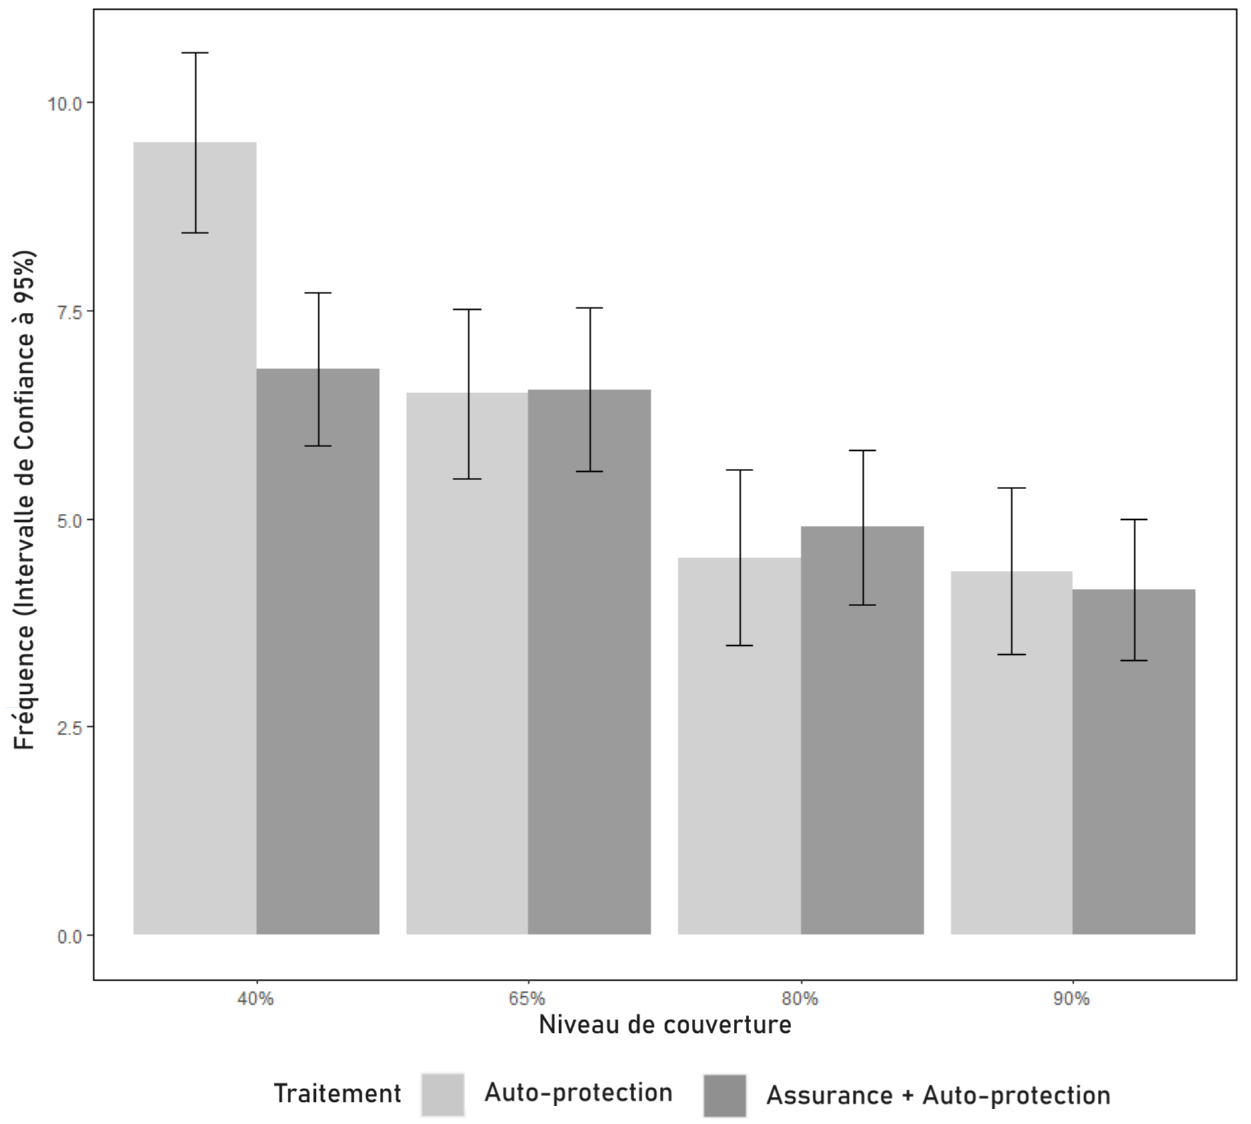
\includegraphics[width=.8\linewidth]{06_insuranceandprevandprev__effort.png}
\end{figure}

À ce stade de l'analyse, un mécanisme de substituabilité entre l'assurance et l'autoprotection semble émerger dans les arbitrages individuels entre ces deux outils de gestion des risques : un plus grand nombre de participants ont choisi des contrats à faible couverture lorsque l'autoprotection était disponible. Ils semblent anticiper leur volonté de réduire la probabilité de perte en utilisant l'autoprotection et décident donc de réduire leur couverture d'assurance dans un premier temps. Ainsi, la décision de réduire la couverture d'assurance dans le traitement \textit{Assurance + autoprotection} pourrait être attribuée à une préférence pour l'autoprotection par rapport à l'assurance, car la disponibilité du mécanisme d'autoprotection est la seule distinction entre les deux traitements.

Afin de confirmer la robustesse de cette hypothèse et, en particulier, de s'assurer que cet effet est bien attribuable à la présence de l'option d'autoprotection et non pas à d'autres paramètres pouvant également influencer les choix d'assurance des individus, trois régressions multivariées ont été estimées. Tout d'abord, un modèle de type logit ordonné à effets aléatoires a été mis en \oe uvre pour estimer le choix d'assurance des participants (modèle 1). Le choix du contrat peut en effet être représenté par une variable catégorielle à quatre modalités, correspondant aux quatre niveaux de couverture disponibles dans chaque menu, avec un ordre sous-jacent (40~\% <~65~\% <~80~\% <~90~\%). Dans ce cadre, le recours à un modèle ordonné à variable latente permet d'identifier l'effet des différents paramètres considérés, y compris la variable de traitement, sur le niveau de couverture choisi par les participants lorsque les choix sont discrets et ordonnés (\textcite{ct05}; \textcite{g11}). Par ailleurs, deux modèles supplémentaires, de type logit à effets aléatoires, ont été effectués pour estimer la probabilité de choisir le contrat avec le taux de couverture le plus bas (40~\%, modèle~2) et le plus élevé (90~\%, modèle 3). Ces deux régressions additionnelles ont été motivées par les résultats descriptifs précédents qui mettent en avant des différences de comportements vis-à-vis des contrats extrêmes et qui sont également les contrats les plus souvent sélectionnés par les participants.

Chacune des trois régressions comprend plusieurs variables de contrôle. Premièrement, deux caractéristiques individuelles ont été incluses : le genre et le niveau d'aversion au risque\footnote{Les variables d'âge et d'éducation ont également été incluses dans les estimations. Compte tenu de la faible variabilité de ces deux variables, les coefficients associés ne ressortent pas significatifs et l'inclusion de ces deux variables n'affecte pas les autres résultats.}. L'aversion au risque est mesurée par le nombre d'options sûres sélectionnées par les participants dans la procédure adaptée du test de \textcite{hl02} au contexte de l'assurance (un participant qui a choisit plus de six options sûres est considéré comme étant averse au risque ; un participant qui choisit huit options sûres est considéré comme plus averse au risque qu'un participant qui en choisit sept)\footnote{Le niveau d'aversion au risque des participants a également été mesuré en considérant le numéro de la question à laquelle ils ont effectué le premier changement d'une option sûre à une option risquée. Les résultats sont similaires puisque 93~\% des sujets sont passés de l'option~A à l'option~B une seule fois ; sur les 7~\% restants, sept sujets ont alternativement choisi les options~A et B (ce qui peut être considéré comme une stratégie de couverture), et un seul participant semble avoir choisi de manière aléatoire (ce participant n'a pas choisi l'option dominante B dans la dernière décision). La majorité de l'échantillon a choisi entre quatre et sept options sûres, ce qui est cohérent avec les résultats trouvés par \textcite{cpm17} en utilisant une procédure similaire.}. Deuxièmement, les caractéristiques de la situation de risque (la probabilité de perte et le montant de la perte) et du menu de contrats d'assurance proposé (le taux de chargement) ont également été prises en compte. Enfin, chaque régression inclut la variable de traitement (\textit{Assurance + autoprotection} \emph{vs} \textit{Assurance}), nécessaire pour estimer l'effet de l'option d'autoprotection sur les choix individuels d'assurance. Le tableau 5 présente les résultats des trois estimations.

% Tableau 5

\begin{table}
  \tabcolsep=2pt
  \caption{Analyses multivariées du choix d'assurance ($\alpha$)}
  \label{tab:insurance_main_results}
  \begin{tabular}[c]{l D{2cm} l D{2cm} l D{2cm} l}
    \toprule
            & \centering Modèle 1 & & \centering Modèle 2 & & \centering Modèle 3 &\tabularnewline
            & \centering Choix d'assurance & & \centering P($\alpha=0,40$) & & \centering P($\alpha=0,90$) &\tabularnewline
    \midrule
    \textbf{\textit{Caractéristiques individuelles}} \\
    \textbf{Genre} \\
    Femme                                & Réf.                             &                         & Réf.                                           &          & Réf.                               &\\
    Homme                                & 0,091 \varstats{0,289}           &                         & 0,784 \varstats{0,356}                         &\sym{**}  & 0,490  \varstats{0,351}            & \\
    \textbf{Aversion au risque}        & 0,118    \varstats{0,099}        &                         & -0,050    \varstats{0,186}                     &          & 0,188    \varstats{0,120}          & \\
    \midrule
    \textit{\textbf{Paramètres du risque}} \\
    \textbf{Probabilité de perte ($\bar{p}$)} \\
    Faible probabilité ($\bar{p}=0,2$)   & Réf.                             &                         & Réf.                                           &          & Réf.                               & \\
    Forte probabilité  ($\bar{p}=0,5$)   & 0,461    \varstats{0,124}        &\sym{***}                & -1,069     \varstats{0,102}                    &\sym{***} & -0,001     \varstats{0,158}        & \\
    \textbf{Montant de perte ($L$)} \\
    Faible perte ($L=600$)               & Réf.                             &                         & Réf.                                           &          & Réf.                               &\\
    Forte perte ($L=1500$)               & 0,645        \varstats{0,124}    &\sym{***}                & -0,546        \varstats{0,100}                 &\sym{***} & 0,648      \varstats{0,160}        &\sym{***}\\
    \midrule
    \textbf{\textit{Caractéristiques du contrat}} \\
    \textbf{Taux de chargement ($\lambda$)} \\
    Nul ($\lambda=0$)                    & Réf.                             &                         & Réf.                                           &          & Réf.                               &\\
    Négatif  ($\lambda=-0,2$)            & 0,331          \varstats{0,151}  &\sym{**}                 & -0,469       \varstats{0,218}                  &\sym{**}  & 0,124       \varstats{0,189}       & \\
    Positif ($\lambda=0,2$)              & -0,424          \varstats{0,150} &\sym{***}                & 0,270      \varstats{0,204}                    &          & -0,715     \varstats{0,199}        &\sym{***}\\
    \midrule
    \textbf{\textit{Traitement}} \\
    \textit{Assurance}                   & Réf.                             &                         & Réf.                                           &          & Réf.                               &\\
    \textit{Assurance + autoprotection} & -0,226        \varstats{0,276}   &                         & 0,715  \varstats{0,330}                        &\sym{**}  & -0,081        \varstats{0,329}     & \\
    \midrule
    Constante                            & -                                &                         & -1,341         \varstats{0,809}                &\sym{*}   & -2,486            \varstats{0,828} &\sym{***}\\
    Seuil 1                              & -0,326        \varstats{0,682}   &                         & -                                              &          & -                                  & \\
    
    Seuil 2                              & 0,831       \varstats{0,682}     &                         & -                                              &          & -                                  & \\
    Seuil 3                              & 1,540         \varstats{0,383}   &\sym{***}                & -                                              &          & -                                  & \\
    \midrule
    \(N\)                                & \multicolumn{2}{c}{960}          & \multicolumn{2}{c}{960} & \multicolumn{2}{c}{960}           \\\bottomrule
    \end{tabular}
    \notedetableau{Significativité : $^{*}$ = 10~\% $^{**}$ = 5~\% $^{***}$ = 1~\%. Les écarts types sont entre parenthèses. Toutes les régressions comprennent des effets aléatoires.}
  \end{table}

  Les résultats révèlent tout d'abord que certaines caractéristiques individuelles, ainsi que celles liées à la situation de risque, affectent les choix d'assurance des participants. Par exemple, même si aucune tendance claire n'est identifiable, le tableau~5 indique une différence entre les choix d'assurance des hommes et des femmes. En particulier, les hommes semblent choisir de moins s'assurer que les femmes, mais avec une différence significative seulement dans la probabilité de sélectionner le contrat avec le taux de couverture le plus bas (modèle~2). De même, conformément à l'intuition qui prévaut en matière de préférence vis-à-vis du risque, un niveau plus important d'aversion au risque semble être associé à des taux de couverture plus élevés (coefficients positifs dans les modèles~1 et 3, et un coefficient négatif dans le modèle~2). Cependant, ce résultat n'est pas statistiquement significatif au seuil de 10~\%. Cette conclusion fait écho à d'autres travaux qui ont montré que le niveau d'aversion au risque joue un rôle limité dans les décisions individuelles d'assurance dans les environnements expérimentaux (\textcite{cpm17}; \textcite{j16}; \textcite{ss11}). Par ailleurs, les caractéristiques du risque ($\bar{p}$ et $L$), ainsi que le taux de chargement ($\lambda$), se révèlent quant à eux des facteurs bien plus déterminants des décisions d'assurance. En particulier, les effets attendus au sens de la théorie économique concernant le montant de la perte et le taux de chargement se retrouvent dans les résultats du tableau 5 : le montant de perte élevé augmente la demande de couverture assurantielle, alors que l'augmentation du taux de chargement tend à la diminuer \parencite{m68}. Enfin, en termes de niveau de risque, alors que les résultats théoriques sont plus ambigus quant à l'effet de la probabilité de perte sur le choix de couverture (\textcite{hr81} ; \textcite{jh95}), la demande d'assurance est plus importante en cas de niveau de risque élevé, dans le cadre de ces données expérimentales.

Concernant spécifiquement l'effet du traitement, il ressort tout d'abord que la présence de l'option d'autoprotection dans le traitement \textit{Assurance + Prévention}, par rapport au traitement \textit{Assurance} dans lequel elle n'est pas proposée, tend à diminuer la probabilité que les individus choisissent un contrat avec un taux de couverture plus important (coefficient négatif dans le modèle~1). Cependant, cet effet n'est pas statistiquement significatif à un seuil de 10~\%. En revanche, une différence significative selon le traitement est observée dans la probabilité de choisir le contrat avec un taux de couverture de 40~\% : l'introduction de l'option d'autoprotection, par rapport au cas où elle n'est pas présente, augmente la probabilité que les participants choisissent le contrat avec le taux de couverture le plus faible (modèle~2), corroborant les résultats descriptifs mis en avant précédemment\footnote{La non-significativité du coefficient associé à la variable de traitement dans le modèle 1 peut s'expliquer par la sur-représentation du taux de couverture de 90\% dans les choix des participants. Cette caractéristique compense l'effet négatif mis en avant dans le modèle~2. De plus, la probabilité de choisir le contrat avec un taux de couverture de 90~\% (modèle~3) est également négative pour les participants du traitement \textit{Assurance + autoprotection} par rapport à ceux du traitement \textit{Autoprotection}, mais non statistiquement significative. À nouveau, la non-significativité de ce coefficient pourrait également être expliquée par le même raisonnement.}.

Ainsi, contrairement à la prédiction théorique (correspondant au résultat attendu principal), les résultats empiriques montrent que l'introduction de l'option d'autoprotection dans le traitement \textit{Assurance + autoprotection} tend à diminuer la demande d'assurance des participants, avec, en particulier, un effet plus marqué sur la probabilité de choisir le contrat avec le taux de couverture le plus faible parmi les options du menu proposé, à autres caractéristiques données. En d'autres termes, lorsque les participants disposent de deux mécanismes de gestion des risques, l'assurance et l'autoprotection, ils vont faire le choix d'acheter moins d'assurance en première étape, par rapport au cas où ils ne disposent que de l'option d'assurance, révélant ainsi un attrait pour l'autoprotection par rapport à l'assurance. Il apparaît donc intéressant de regarder comment cette déviation par rapport à la prédiction théorique, qui ne prévoit pas de changement en matière de choix d'assurance avec ou sans l'option d'autoprotection, se traduit en termes d'effort d'autoprotection. En particulier, est-ce que ce changement de comportement se traduit ensuite par davantage d'efforts d'autoprotection ? Il s'agit ici de tester la cohérence empirique des arbitrages individuels entre l'assurance et l'autoprotection.


\subsection{Incohérence des comportements entre les deux étapes\\ de l'expérimentation}
\label{section:H2selfpro}

Pour analyser et comprendre les décisions individuelles en matière\linebreak d'autoprotection, et surtout examiner si leur choix d'assurance, effectué au préalable, se répercute sur l'effort que les participants consentent à fournir, il est nécessaire de distinguer deux effets : l'effet propre du niveau de couverture (effet de l'aléa moral) et l'effet d'un réel arbitrage individuel entre l'assurance et l'autoprotection. Pour ce faire, un troisième traitement a été mis en \oe uvre, le traitement\textit{ Autoprotection}. Ce traitement, qui consiste à attribuer de manière aléatoire un contrat d'assurance parmi les quatre figurant dans le menu, va permettre d'observer les comportements d'effort d'autoprotection des participants en réaction à la souscription d'un contrat d'assurance donné, afin de capter l'effet propre du niveau de couverture sur le niveau d'effort fourni en seconde étape. Par comparaison avec le traitement \textit{Assurance + autoprotection}, il sera ainsi possible de distinguer l'effet relevant exclusivement du taux de couverture du contrat d'assurance, assimilable à un effet en termes d'aléa moral en cas de diminution de l'effort d'autoprotection avec l'augmentation du taux de couverture attribué, de celui qui relèverait d'une stratégie de diversification entre l'assurance et l'autoprotection comme escompté à partir des résultats précédents (à savoir, est-ce qu'un niveau de couverture plus faible, choisi dans la première étape (résultat précédent), se traduit par un effort d'autoprotection accru dans la deuxième étape ?).

La figure 2 reporte le niveau moyen d'effort d'autoprotection des participants ($e$), en fonction du niveau de couverture assurantielle, selon le traitement (ce taux de couverture est choisi par les participants dans le cas du traitement \textit{Assurance + autoprotection} et imposé dans le cas du traitement \textit{Autoprotection}). Tout d'abord, les niveaux d'effort d'autoprotection observés dans le cadre du traitement \textit{Autoprotection} uniquement, semblent valider l'hypothèse d'un effet d'aléa moral, marqué par une diminution du niveau d'effort avec l'augmentation du taux de couverture imposé aux participants. Par ailleurs, un test non paramétrique de Kolmogorov-Smirnov indique une différence significative globale dans la distribution de $e$ entre les deux traitements (\textit{p-value} = 0,006). Plus précisément, cette différence provient de l'écart significatif d'effort d'autoprotection observé pour le contrat d'assurance disposant du niveau de couverture le plus faible (40~\%). La figure~2 montre clairement que les individus qui ont choisi le contrat avec un taux de couverture de 40~\% (traitement \textit{Assurance + autoprotection}), font en moyenne moins d'effort d'autoprotection que ceux pour qui ce même contrat a été imposé (traitement \textit{Autoprotection}).
 
D’un point de vue théorique, les décisions individuelles en matière d’assurance et d’autoprotection sont indépendantes. Ainsi, aucune différence, en termes de niveau de couverture assurantielle, ne devrait être observée entre les traitements\textit{ Assurance} et \textit{Assurance + autoprotection} ; de même qu’aucune différence ne devrait apparaître entre les traitement \textit{Autoprotection} et \textit{Assurance + autoprotection} en termes d’effort d’autoprotection. Pourtant, les résultats expérimentaux précédents invalident la première prédiction puisqu'une augmentation de la probabilité de sélectionner le contrat le moins complet (40~\%) est observée lorsque l'option d'autoprotection est disponible, par rapport au cas où elle ne l'est pas. Ainsi, si cette régularité empirique s’explique par une préférence pour l’autoprotection par rapport à l’assurance et que les participants restent cohérents dans leur arbitrage entre les deux outils de gestion des risques, des efforts d’autoprotection supérieurs --~bien que contraires aux prédictions théoriques~-- devraient être observés dans le traitement \textit{Assurance + autoprotection}, par rapport au traitement \textit{Autoprotection} (qui pourrait s'interpréter comme  une augmentation compensatrice consécutive à la décision de réduire sa couverture assurarielle). Or, la figure~2 semble contredire cette hypothèse.

% Figure 2

\begin{figure}[h!]
\caption{Niveau moyen d’effort d’autoprotection (e) en fonction du traitement}
  \centering
  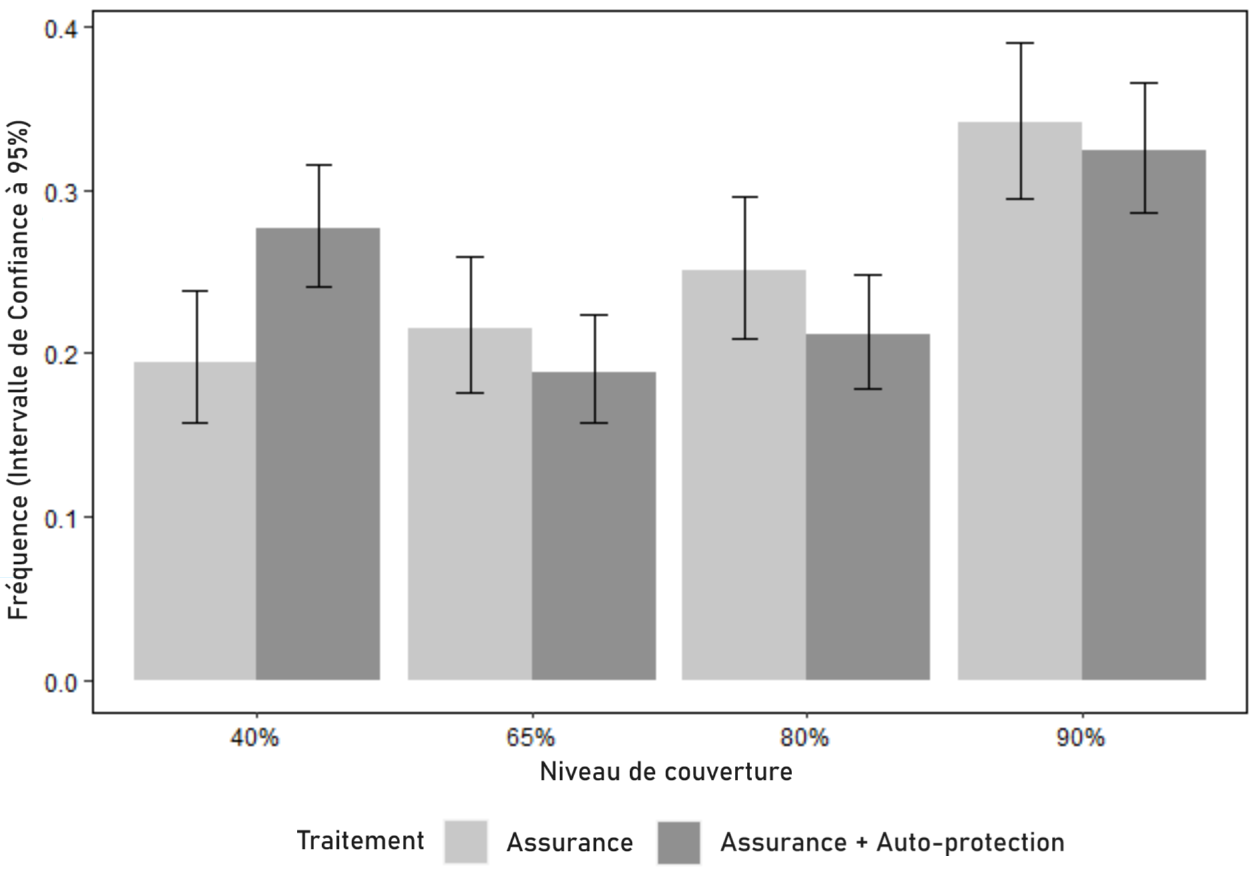
\includegraphics[width=.8\linewidth]{Articles-bons-a-composer/06_Mouminoux_al/06_Mouminoux_Figures/06_distrib_couv_treatment_english.png}
\end{figure}

Pour affiner ces résultats descriptifs, un modèle de régression linéaire à effets aléatoires a été utilisé afin d'estimer le niveau d'effort d'autoprotection $e$ choisi par les participants dans les traitements \textit{Assurance + autoprotection} et \textit{Autoprotection}. La régression inclut, à nouveau, toutes les caractéristiques observables décrites précédemment (caractéristiques individuelles, paramètres du risque et caractéristiques du contrat d'assurance). De plus, trois variables binaires correspondant au niveau de couverture assurantielle dont disposent les participants avant d'effectuer leur effort d'autoprotection --~soit choisi, soit imposé~-- sont également incluses afin de contrôler l'effet propre du taux de couverture sur l'effort d'autoprotection (l'effet de l'aléa moral). Par ailleurs, afin de distinguer l'effet d'aléa moral de celui d'un arbitrage individuel entre l'assurance et l'autoprotection, des termes d'interaction entre chaque niveau de couverture et la variable de traitement ont été ajoutés. Ces variables permettent de tester si la relation entre le niveau de couverture et le niveau d'effort d'autoprotection est la même lorsque le contrat est préalablement choisi par les participants (traitement \textit{Assurance + autoprotection}) ou attribué de manière exogène (traitement \textit{Autoprotection}). Ainsi, si la préférence pour l'autoprotection observée précédemment se traduit par davantage d'efforts d'autoprotection ensuite, un coefficient positif associé au terme d'interaction entre le niveau de couverture à 40~\% et le traitement \textit{Assurance + autoprotection} devrait être observé. Le tableau 6 présente les coefficients estimés.

Tout d'abord, les résultats révèlent une corrélation négative entre le niveau d'assurance et le niveau d'autoprotection, qui se traduit par moins d'efforts d'autoprotection dans le cas de taux de couverture plus élevés, toutes choses étant égales par ailleurs et, en particulier, indépendamment du traitement. En effet, la diminution du taux de couverture, notamment pour les cas des contrats avec les taux de couverture de 40~\% et 65~\%, implique un effort d'autoprotection plus important par rapport au cas des contrats plus complets. Ce premier résultat est conforme à l'hypothèse d'un effet d'aléa moral formulée dans la théorie économique. De même, il est également conforme au résultat obtenu par \textcite{eb72}, dans le cadre d'un modèle à une période, démontrant que l'assurance et l'autoprotection sont des substituts lorsque la prime d'assurance ne prend pas en compte l'effort d'autoprotection.

% Tableau 6

\newpage

\begin{table}[h!]
\caption{Analyses multivariées du niveau d'effort d'autoprotection $e$}
\label{tab:sp_main_results}
\centering
\resizebox{!}{0.45\textheight}{
\begin{tabular}{lrl}
\toprule
   & $e$ & \\
\midrule
\textit{\textbf{Caractéristiques individuelles}} & & \\
\textbf{Genre} & & \\
Femme  & Réf. & \\
Homme  & 1,126 & \\
       & \varstats{0,778} & \\
\textbf{Aversion au risque} & -0,367 & \\
       & \varstats{0,319} & \\
\textit{\textbf{Paramètres du risque}} & & \\
\textbf{Probabilité de perte ($\bar{p}$)} & & \\
Faible probabilité ($\bar{p}=0,2$) & Réf. & \\ 
Forte probabilité ($\bar{p}=0,5$) & 0,646 & \sym{**}  \\
    & \varstats{0,290} & \\
\textbf{Montant de la perte ($L$)} &  &\\
Faible perte ($L=600$) & Réf. & \\
Forte perte ($L=1 500$) & -1,700 & \sym{***} \\
    & \varstats{0,290} & \\
\textit{\textbf{Caractéristiques du contrat}} & & \\
\textbf{Taux de chargement ($\lambda$) } & & \\
Nul ($\lambda=0$)  & Réf. & \\
Négatif ($\lambda=-0,2$) & 0,739 & \sym{**} \\
   & \varstats{0,352} & \\
Positif ($\lambda=0,2$) & 0,748 & \sym{**} \\
   &  \varstats{0,351} & \\
\textbf{Taux de couverture ($\alpha$)} & & \\
40~\% & Réf. & \\
65~\% & -2,609 & \sym{***}\\
     & \varstats{0,588} & \\
80~\% & -3,782 & \sym{***} \\
     & \varstats{0,653} & \\
90~\% & -4,619 & \sym{***} \\
     & \varstats{0,595} &  \\
\textbf{Taux de couverture $\times$ Traitement} \\
40~\% $\times$ Traitement \textit{Assurance + autoprotection} & -1,602 & \sym{*} \\
         &     \varstats{0,909} & \\
65~\% $\times$ Traitement \textit{Assurance + autoprotection} & 0,359 & \\
         &     \varstats{0,934} & \\
80~\% $\times$ Traitement \textit{Assurance + autoprotection} & -0,228 & \\
         &     \varstats{0,953} & \\
90~\% $\times$ Traitement \textit{Assurance + autoprotection} & -0,933 & \\
         &     \varstats{0,889} & \\
\midrule
Constante   &  10,458 & \sym{***} \\
            &  \varstats{2,073} & \\
\(N\)           &  1080 &  \\
\bottomrule
\end{tabular}}
\notedetableau{Significativité : $^{*}$ = 10~\%, $^{**}$ = 5~\%, $^{***}$ = 1~\%. Les écarts types sont entre parenthèses. La régression inclut des effets aléatoires.}
\end{table}

Au-delà de la corrélation négative globale observée entre le niveau de couverture et le niveau d'autoprotection, le résultat central concerne la nature de cette relation en fonction du traitement. En particulier, les résultats montrent que les participants du traitement \textit{Assurance + autoprotection}, qui ont choisi le niveau de couverture de 40~\%, ne fournissent pas un effort d'autoprotection plus important en deuxième étape, par rapport aux participants du traitement \textit{Autoprotection} ($p < 0,10$ associée au terme d'interaction entre le taux de couverture à 40~\% et la variable de traitement). Au contraire, ils fournissent moins d'efforts que les participants à qui ce contrat a été attribué de manière exogène. Pour les autres niveaux de couverture, aucune différence significative dans l'effort d'autoprotection n'est observée selon le groupe de traitement.

Finalement, les participants qui ont choisi d'être moins assurés lors de la première étape dans le traitement \textit{Assurance + autoprotection}, révélant ainsi un attrait pour l'autoprotection, ne fournissent pas plus d'efforts d'autoprotection par la suite (le coefficient négatif suggère même un comportement opposé). Alors que ce résultat est basé sur la comparaison des niveaux d'effort des participants entre les traitements \textit{Assurance + autoprotection} et \textit{Autoprotection}, l'une des interprétations possibles tient à l'existence d'un potentiel effet d'offre lié à l'environnement expérimental du laboratoire \parencite{clv10}. En retirant la possibilité de choisir le contrat d'assurance aux participants dans le traitement \textit{Autoprotection}, faisant ainsi de l'autoprotection le seul outil de gestion du risque manipulable par les participants, ce design pourrait avoir pour effet d’inciter les individus à fournir davantage d’effort d'autoprotection, quel que soit le taux de couverture du contrat attribué (le sujet expérimenté choisirait de faire un effort en raison de sa seule volonté d'apparaître actif lors de l’expérimentation). Pour tester cette hypothèse, il a été question de comparer la probabilité, pour les participants, de ne fournir aucun effort d'autoprotection ($e=0$), entre les deux traitements \textit{Assurance + autoprotection} et \textit{Autoprotection}\footnote{Pour ce faire, un modèle de type logit à effets aléatoires a été utilisé pour estimer la probabilité de ne fournir aucun effort d'autoprotection en fonction du traitement, tout en contrôlant des autres caractéristiques observables.}. Les résultats, reportés dans le tableau~A2 en annexe~\ref{Annexe:supply_effect}, ne semblent pas
valider cette hypothèse puisque la différence dans la probabilité que les participants ne fassent aucun effort ($e = 0$) entre les deux traitements n'est pas statistiquement significative. L’hypothèse d’un  effet d'offre pour expliquer ce résultat est donc peu crédible ici.

En résumé, les résultats ont mis en évidence des comportements individuels différents des prédictions théoriques dictées par la théorie de l'utilité espérée, et marqués par une forme d'incohérence entre deux décisions ayant lieu de manière séquentielle (entre les deux étapes de l'expérimentation). Ce résultat peut être mis en relation avec certains travaux en psychologie sociale, à l'instar de ceux de \textcite{abc04}, qui montrent le rôle majeur du concept de biais hypothétique dans la formation des écarts entre les intentions déclarées des individus et les actions qu'ils entreprennent finalement. Selon l'hypothèse de la présence de biais hypothétiques, l'idée que les individus sont capables de planifier correctement leurs décisions dans un environnement dynamique pourrait être remise en question (la théorie du comportement planifié \parencite{Ajzen1991}). L'expérimentation est conçue de telle sorte que l'effort d'autoprotection n'est qu'hypothétique au moment où les participants choisissent leur contrat d'assurance. En effet, lorsque les deux mécanismes coexistent (traitement \textit{Assurance + autoprotection}), l'étape 1 consiste, pour chaque participant, à choisir un contrat d'assurance sachant que l'autoprotection est disponible ensuite (mais n'apparaît pas encore à l'écran). Le mécanisme d'autoprotection ne devient tangible qu'une fois le contrat souscrit, lors de la seconde étape du jeu (la souscription du contrat d'assurance conduit à l'écran suivant qui affiche l'étape~2). Ainsi, la validation du choix de l'assurance met fin au biais hypothétique et cède la place à l'action d'autoprotection, qui révèle alors la nature de l'incohérence des choix observés. Cette disconnexion entre la préférence et les efforts réellement entrepris a été observée dans plusieurs travaux empiriques. Par exemple, dans le contexte de la santé, \textcite{öjh09} montrent que la volonté des individus à payer pour un traitement médical donné est plus grande que ce qu'ils paient réellement. En utilisant des données expérimentales, \textcite{ms04} analysent les comportements individuels à travers la notion de conformité (ou observance) à un traitement médical et révèlent une différence entre l'acceptation hypothétique et réelle du traitement. \textcite{qtdv18} passent en revue la littérature et mettent en évidence des écarts entre les préférences de santé déclarées (expériences de choix discrets\footnote{Outil économique utilisé pour solliciter les préférences déclarées des répondants.}) et les comportements. Tous ces exemples, qui présentent tous une différence entre les intentions déclarées et les actions entreprises, soulignent l'importance du rôle joué par le biais hypothétique \parencite{hrg15}, et qui pourrait en partie expliquer les résultats expérimentaux obtenus dans cette étude.


\section{Discussion et conclusion}
\label{section:conclusion}

Cette étude repose sur un protocole expérimental ayant pour objectif d'analyser les comportements individuels dans des situations risquées, où l'assurance et l'autoprotection coexistent. À partir de deux traitements expérimentaux différents, les choix individuels en matière d'assurance ont pu être comparés selon que les participants aient, ou non, accès à une option d'autoprotection après avoir souscrit leur contrat d'assurance. Cette première analyse a mis en évidence une relation de substituabilité entre l'assurance et l'autoprotection, marquée par une préférence pour l'autoprotection par rapport à l'assurance. En effet, les individus ont opté pour des contrats moins complets lorsque l'option d'autoprotection était accessible. Par ailleurs, l'implémentation d'un troisième traitement, dans lequel le contrat d'assurance était imposé de façon aléatoire, a ensuite permis d'examiner les efforts d'autoprotection fournis par les individus en deuxième étape et, en particulier, de tester la cohérence des choix séquentiels entre l'assurance et l'autoprotection. Les résultats indiquent que les individus qui semblaient exprimer une préférence pour l'autoprotection à travers leurs choix d'assurance, ne semblent pas fournir davantage d'efforts d'autoprotection une fois rendus à la deuxième étape du jeu. En d'autres termes, l'attrait pour l'autoprotection n'implique pas davantage d'efforts d'autoprotection une fois que le coût de l'effort devient réel.

Ces résultats expérimentaux s'inscrivent dans la continuité des travaux portant sur la question de l'arbitrage entre l'assurance et l'autoprotection. Alors que la plupart de ces travaux ont expliqué la substituabilité entre ces deux outils de gestion des risques par l'effet dissuasif de l'assurance sur l'autoprotection (effet d'aléa moral), cette étude montre que l'introduction d'une option d'autoprotection peut également réduire la demande d'assurance. Dans ce contexte, le développement de contrats d'assurance incluant une option d'autoprotection doit prendre en compte ce résultat pour anticiper d'éventuels comportements de sous-assurance. Cette conclusion est d'autant plus préoccupante compte tenu du deuxième résultat de ce travail, qui révèle que les individus qui semblent exprimer une préférence pour l'autoprotection par rapport à l'assurance ne sont finalement pas enclins à fournir davantage d'efforts d'autoprotection lorsqu'ils sont confrontés au coût réel de cet effort. Ainsi, l'un des principaux défis auxquels les décideurs doivent faire face concerne la motivation à s'engager réellement dans l'autoprotection.

Finalement, bien que l'autoprotection reste souhaitable d'un point de vue global, l'incohérence dans la prise de décisions des individus lorsque plusieurs outils de gestion des risques coexistent soulève de nouvelles questions. Par exemple, comment limiter les effets indésirables et améliorer l'efficacité de l'autoprotection ? \textcite{ArielyWertenbroch2002} soutiennent que la nature auto-contraignante d'une décision pourrait limiter la divergence entre les intentions et les actions, ce qui pourrait être une approche intéressante à adopter. Cependant, contraindre les assurés à s'engager dans l'autoprotection révèle ses propres limites, telles que la nécessité de mettre en place des moyens de contrôle ou encore l'éventualité d'effets d'éviction. Par conséquent, encourager les activités d'autoprotection à travers des campagnes de sensibilisation reste l'un des moyens les plus efficaces de sensibiliser aux risques. Cependant, une attention particulière doit être portée aux comportements de sous-assurance potentiels que les véritables efforts d'autoprotection ne compensent pas.

\printbibliography

\begin{appendices}
  
\section{Instructions}
\label{Annexe:Instruction}

\begin{figure}[htbp]
  \centering
  \includegraphics[page=1,scale=0.6]{Articles-bons-a-composer/06_Mouminoux_al/06_Mouminoux_Figures/06_Protocole.pdf}
\end{figure}

\begin{figure}[htbp]
  \centering
  \includegraphics[page=2,scale=0.6]{Articles-bons-a-composer/06_Mouminoux_al/06_Mouminoux_Figures/06_Protocole.pdf}
\end{figure}

\begin{figure}[htbp]
  \centering
  \includegraphics[page=3,scale=0.6]{Articles-bons-a-composer/06_Mouminoux_al/06_Mouminoux_Figures/06_Protocole.pdf}
\end{figure}

\begin{figure}[htbp]
  \centering
  \includegraphics[page=4,scale=0.6]{Articles-bons-a-composer/06_Mouminoux_al/06_Mouminoux_Figures/06_Protocole.pdf}
\end{figure}

\begin{figure}[htbp]
  \centering
  \includegraphics[page=5,scale=0.6]{Articles-bons-a-composer/06_Mouminoux_al/06_Mouminoux_Figures/06_Protocole.pdf}
\end{figure}

\begin{figure}[htbp]
  \centering
  \includegraphics[page=6,scale=0.6]{06_Protocole.pdf}
\end{figure}

\newpage

\section{Résultats attendus}
\label{Annexe:Expected_results}

\subsection{Résultats théoriques}
\label{Annexe:Expected_results_theo}

\paragraph*{Cas 1 : Individus neutres au risque}

Les individus neutres au risque se caractérisent par une fonction d'utilité $U(.)$ linéaire et strictement croissante, et sont supposés maximiser le programme suivant :

\begin{equation}
\left\{
    \begin{array}{ll}
    \displaystyle \max_{\alpha,e} ~~ W - e -\alpha(1+\lambda)\bar{p}L - (\bar{p}-a\cdot e)(1 - \alpha)L\\
    \text{s.c.} ~~0 \le e \le \bar{e}\enskip \text{et}\enskip \underline{\alpha} \le \alpha \le \bar{\alpha}
    \end{array}
\right.
\end{equation}

\noindent avec $\underline{\alpha}$ et $\bar{\alpha}$, respectivement les taux de couverture d'assurance minimum et maximum proposés dans chaque menu de contrats et $\bar{e}$ le niveau d'effort maximum d'autoprotection.

Étant donné que $\alpha$ et $e$ sont des variables de décision prises séquentiellement dans le traitement \textit{Assurance + autoprotection} (choix de $\alpha$ puis de $e$), le recours à un raisonnement par induction récursive (\textit{backward induction}) est nécessaire pour résoudre ce programme d'optimisation. La démarche consiste à déterminer, dans un premier temps, le niveau d'effort d'autoprotection optimal, $e^*(\alpha)$, $\forall\alpha>0$ (étape 1), puis de déterminer le niveau de couverture optimal $\alpha^*$ en fonction de $e^*$, c'est-à-dire en remplaçant $e$ par $e^*(\alpha)$ dans le programme d'optimisation (étape 2). \\

\textit{Étape 1}\footnote{Cette étape correspond également à la résolution du traitement \textit{Autoprotection}.}   \\

Soit $CP=\alpha(1+\lambda)\bar{p}L$ et $D=(1 - \alpha)L$. Ainsi :
\begin{equation}
\left\{
    \begin{array}{ll}
e^* = \arg\max W - e - CP - (\bar{p}-a\cdot e)D = \arg\max e \cdot (aD-1) \\
      \text{s.c.} ~~0 \le e \le \bar{e}
    \end{array}
\right.
\end{equation}

La solution de ce problème d'optimisation consiste à trouver le signe de $(aD-1)$, soit encore le signe de $a(1-\alpha )L-1$, sachant que $D=(1 - \alpha)L$\footnote{En effet, si $(aD-1)=0$ le décideur est indifférent entre les différents niveaux de $e$ (soit $e^*\in [0;\bar{e}]$), si $(aD-1)>0$ alors $e^*=\bar{e}$, et si $(aD-1)<0$ alors $e^*=0$.}.

Sachant que $a=\frac{1}{L}$, étant donné que le coût de l'effort est calculé de sorte que réduire la probabilité de perte à 0 en utilisant l'autoprotection représente le même coût que la souscription d'une assurance complète au prix actuariel, et que l'assurance est obligatoire ($\alpha > 0$), on a :
\begin{equation}
\frac{1}{L}(1-\alpha )L-1=-\alpha<0.
\end{equation}

Ainsi, on obtient $e^*(\alpha)=0,~ \forall \alpha>0$.

\clearpage

\textit{Étape 2} \\

En remplaçant $e$ par $e^*(\alpha)$, on obtient le programme d'optimisation suivant :
\begin{equation}
\left\{
    \begin{array}{ll}
\alpha^* = \arg\max W - CP - \bar{p}D = \arg\max W - \alpha(1+\lambda)\bar{p}L - \bar{p}(1 - \alpha)L \\
\Leftrightarrow \alpha^* = \arg\max ~ -\lambda \alpha \\
    \text{s.c.} ~~\underline{\alpha} \leq \alpha \leq \bar{\alpha}.
    \end{array}
\right.
\end{equation}

Par conséquent, et conformément au modèle de \textcite{m68}, le niveau de couverture optimal pour un individu neutre vis-à-vis du risque dépendra uniquement du signe de $\lambda$, tel que :
\begin{itemize}
  \item Si $\lambda>0$, alors $\alpha^*=\underline{\alpha}$,
  \item Si $\lambda=0$, alors $\alpha^* \in [\underline{\alpha},\bar{\alpha} ]$,
  \item Si $\lambda<0$, alors $\alpha^*=\bar{\alpha} $.
\end{itemize}

\paragraph*{Cas 2 : Individus risquophiles}

Les individus risquophiles se caractérisent par une fonction d'utilité $U(.)$ convexe et strictement croissante, et sont supposés maximiser le programme suivant :
\begin{equation}
\left\{
    \begin{array}{ll}
   \displaystyle \max_{\alpha, e} ~~EU(\alpha,e)=(\bar{p}-a\cdot e)U[W - e -\alpha(1+\lambda)\bar{p}L - (1 - \alpha)L] \\
   + (1 - \bar{p}+a\cdot e)U[W - e - \alpha(1 + \lambda)\bar{p}L] \\
     \text{s.c.} ~~0 \le e \le \bar{e}\enskip \text{et}\enskip \underline{\alpha} \le \alpha \le \bar{\alpha}
    \end{array}
\right.
\end{equation}

\noindent avec $\underline{\alpha}$ et $\bar{\alpha}$, respectivement les taux de couverture d'assurance minimum et maximum proposés dans chaque menu de contrats et $\bar{e}$ le niveau d'effort maximum d'autoprotection.

Le raisonnement par induction récursive est à nouveau utilisé pour déterminer $e^*(\alpha), \forall\alpha>0$ (étape 1), puis $\alpha^*$ (étape 2). \\

\textit{Étape 1} \\

On considère la condition de premier ordre (CPO), soit :
\begin{multline}
\frac{\partial EU(\alpha, e)}{\partial e}=0\Leftrightarrow a(U[W - CP -e] -U[W - CP -D -e]) \\
=(\bar{p}-a\cdot e)U'[W - CP -D -e]+(1 - \bar{p}+a\cdot e)U'[W - CP -e].
\end{multline}

On considère ensuite la condition de second ordre (CSO), soit :
\begin{equation}
\frac{\partial EU(\alpha, e)^2}{\partial e^2}=(\bar{p}-a\cdot e)U''[W - CP -D -e]+(1 - \bar{p}+a\cdot e)U''[W - CP -e].
\end{equation}

Étant donné que $U''(.)>0$, $e^*$ est une solution en coin, telle que $e^* \in \{0;\bar{e}\}$.
Par ailleurs, sachant que $U(.)$ est une fonction strictement croissante et convexe, que la souscription à un contrat d'assurance est obligatoire et que la couverture complète n'est pas disponible ($0<\alpha<1$), en utilisant l'inégalité de Jensen, on a :
\begin{multline}
EU(\alpha, 0)= \bar{p}U[W  -CP - D] + (1 - \bar{p})U[W - CP] \\
> U[\bar{p}\times (W  -CP -D) + (1 - \bar{p}) (W - CP)] = U[W-CP-\bar pD].
\end{multline}

Avec $EU(\alpha, \bar e)=(\bar{p}-a\cdot \bar e)U[W - \bar e -CP - D] + (1 - \bar{p}+a\cdot \bar e)U[W - \bar e - CP],$ soit :
\begin{multline}
EU(\alpha, 0)-EU(\alpha, \bar e) \\
> U[W-CP-\bar pD]-(\bar{p}-a\cdot \bar e)U[W - \bar e -CP - D]- (1 - \bar{p}+a\cdot \bar e)U[W - \bar e - CP] \\
> U[W-CP-\bar pD]-(\bar{p}-a\cdot e)U[W - \bar e -CP - D]- (1 - \bar{p}+a\cdot \bar e)U[W - \bar e - CP-D] \\ 
\Rightarrow EU(\alpha, 0)-EU(\alpha, \bar e) \\
>U[W-CP-\bar pD]-U[W - \bar e -CP - D]>0
\end{multline}

\noindent avec $U(.)$ une fonction strictement croissante et $W-CP-\bar pD>W - \bar e -CP - D \Leftrightarrow \bar e+D>\bar pD \Leftrightarrow e>D(\bar p-1) $ puisque $\bar e>0$, on a donc :
\begin{equation}
EU(\alpha, 0)>EU(\alpha, \bar e),~\forall\alpha~;~ 0<\alpha<1.
\end{equation}

Par conséquent, l'effort optimal d'autoprotection est toujours nul pour les individus risquophiles (soit $e^*(\alpha)=0$) lorsque l'assurance est obligatoire et que la couverture complète n'est pas disponible ($0<\alpha<1$). \\

\textit{Étape 2} \\

La deuxième étape consiste à déterminer $\alpha^*$ sachant $e^*$. Pour ce faire, on considère à nouveau les conditions de premier et second ordre. Soit :
\begin{multline}
\frac{\partial EU(\alpha, e^*)}{\partial \alpha}=0 \\
\Leftrightarrow  (\bar{p}-a\cdot e^*)(-(1+\lambda)\bar{p}L+L)U'[W - e^* -\alpha(1+\lambda)\bar{p}L - (1 - \alpha)L] \\
 + (1 - \bar{p}+a\cdot e^*)(-(1 + \lambda)\bar{p}L)U'[W - e^* - \alpha(1 + \lambda)\bar{p}L]=0.
\end{multline}

Puis :
\begin{multline}
\frac{\partial EU(\alpha, e^*)^2}{\partial \alpha^2}=(\bar{p}-a\cdot e^*)(-(1+\lambda)\bar{p}L+L)^2U''[W - e^* -\alpha(1+\lambda)\bar{p}L - (1 - \alpha)L] \\
+(1 - \bar{p}+a\cdot e^*)(-(1 + \lambda)\bar{p}L)^2U''[W - e^* - \alpha(1 + \lambda)\bar{p}L].
\end{multline}

Sachant que $e^*=0$ et que $U''(.)>0$, cela implique que $\alpha^*$ est également une solution en coin, telle que $\alpha^* \in \{\underline{\alpha};\bar{\alpha}\}$.

En utilisant la CSO et étant donné que $U(.)$ est une fonction strictement croissante ($U'(.)>0$), on peut montrer que pour tout $\lambda \geq 0$, un individu risquophile choisira le taux de couverture le plus faible disponible lorsque l'assurance est obligatoire, soit $\alpha^*=\underline{\alpha}$. En effet, on a :
\begin{multline}
\frac{\partial EU(\alpha, 0)}{\partial \alpha}=-\lambda\bar{p}L[\bar{p}U'[W -CP-D]+(1 - \bar{p})U'[W -CP]] \\
-(1 - \bar{p})U'[W -CP]<0, ~\forall \lambda \geq 0 ,~\forall \overline \alpha >\alpha >\underline \alpha.
\end{multline}

Cependant, puisque le cas où $\lambda<0$ n'est pas exclu (cas d'une assurance subventionnée), un individu modérément risquophile peut avoir un intérêt à choisir la couverture maximale si l'assurance est suffisamment subventionnée.
Dans ce cadre, on a :
\begin{multline}
\frac{\partial EU(\alpha, 0)}{\partial \alpha}=\bar{p}(-(1+\lambda)\bar{p}L+L)U'[W -CP - D] \\
+ (1 - \bar{p})(-(1 + \lambda)\bar{p}L)U'[W - CP] >0, ~\forall \lambda \leq -1 ,~\forall \overline \alpha >\alpha >\underline \alpha. 
\end{multline}

La prime d'assurance est supposée toujours positive, soit $\lambda>-1$. Étant donné que $\frac{\partial EU(\alpha, 0)}{\partial \alpha}<0,~\forall \lambda \geq 0$ et $\frac{\partial EU(\alpha, 0)}{\partial \alpha}>0, ~\forall \lambda \leq -1$, et puisque $\frac{\partial EU(\alpha, 0)}{\partial \alpha}$ est continue en $\lambda$ ; en utilisant le théorème des valeurs intermédiaires, on peut montrer qu'il existe un $\bar{\lambda}$ tel que $0 > \bar{\lambda} > -1$, où $\frac{\partial EU(\alpha, 0)}{\partial \alpha}$ peut être soit positive soit négative en fonction de la valeur de $\alpha$. Ainsi, lorsque $0 > \lambda > -1$, il est nécessaire de comparer l'utilité espérée pour $\alpha^* \in \{\underline{\alpha}, \overline{\alpha}\}$. En particulier, la solution est forcément une solution en coin, qui dépend de la valeur de $\lambda$, avec $\frac{\partial \alpha^*}{\partial \lambda} \le 0$.

\paragraph*{Cas 3 : Individus averses au risque}

Les individus averses au risque se caractérisent par une fonction d'utilité $U(.)$ concave et strictement croissante, et sont supposés maximiser le même programme que celui décrit dans le cas 2 (individus risquophiles). De même, les conditions de premier et second ordre sont les mêmes que celles décrites dans le cas précédent. En revanche, pour le cas des individus averses au risque, on a $U''(.)<0$. Ainsi, la CPO devient suffisante et $e^*$ satisfait la relation suivante : 
\begin{multline}
 a(U[W - CP -e^*] -U[W - CP -D -e^*]) \\
 = (\bar{p}-a\cdot e^*)U'[W - CP -D -e^*] \\
 +(1 - \bar{p}+a\cdot e^*)U'[W - CP -e^*].
\end{multline} 
 
Cependant, il est tout de même nécessaire de vérifier que la solution est une solution intérieure, telle que $e^* \in [0, \overline{e}]$. Si ce n'est pas le cas, étant donné que $e$ prend des valeurs sur un intervalle borné fermé, la solution est une solution en coin.

À ce stade, il est nécessaire de spécifier une forme spécifique de fonction d'utilité, ainsi que des valeurs de paramètres associés, pour obtenir une expression explicite de $e^*$ et $\alpha^*$.


\subsection{Calculs numériques}
\label{Annexe:Expected_results_num}

Bien qu'il soit généralement admis que les individus présentent une aversion absolue au risque décroissante (fonction d'utilité de type DARA), il n'y a pas de consensus parmi les économistes concernant l'aversion relative au risque des individus. \textcite{o14} détaille les différentes conclusions sur l'aversion relative au risque dans la littérature sur la demande d'assurance. Alors que l'utilisation d'une fonction d'utilité avec une aversion au risque relative constante (fonction d'utilité de type CRRA) peut être justifiée selon certaines définitions de la richesse, les individus présentent souvent une aversion relative au risque décroissante (fonction d'utilité de type DRRA), ce qui indique qu'ils deviennent plus tolérants au risque à mesure que leur richesse ou leur niveau de couverture augmente, ce qui peut les amener à opter pour une couverture d'assurance plus faible ou des franchises plus élevées. Ainsi, comme le suggèrent \textcite{hl02}, nous utilisons une fonction d'utilité de type \og\textit{power-expo}\fg, proposée par \textcite{s93}, pour vérifier les résultats précédents dans le cas d'une aversion relative au risque décroissante (fonction d'utilité de type DRRA). Pour ce faire, on considère la fonction d'utilité suivante :
\begin{equation}
U(x) = \theta -e^{-\beta x^\alpha}.
\end{equation}

Les choix théoriques, sous l'hypothèse d'une aversion relative au risque décroissante (fonction d'utilité de type DRRA), sont calculés selon une large gamme de paramètres de la fonction d'utilité, en considérant $\alpha \in [-3,0[$ et $\beta \in [-3,0[$\footnote{$\theta$ est une constante et ne modifie pas les choix lors de la comparaison des loteries selon la théorie de l'utilité espérée.}. Les mêmes résultats précédemment décrits pour l'aversion au risque relative constante (fonction d'utilité de type CRRA) restent valables. De plus, nous constatons que ces résultats sont également valables lorsque l'on considère une aversion relative au risque croissante (fonction d'utilité de type IARA) avec des valeurs de paramètres raisonnables : $0 < \alpha < 1$ et $\beta \in ]0,~3]$, avec $\alpha\beta<0,05$ (par exemple, $\hat{\beta}=0,029$ dans \textcite{hl02}).

\section{Élicitation de l'aversion au risque\\ dans le domaine des pertes}

\label{Annexe:Holt_Laury}

\begin{table}[!h]
    \tabcolsep=3pt
    \centering
\caption{Élicitation de l'aversion au risque}
\label{tab:Holt_Laury}
\begin{tabular}[c]{c|rcrc|c|rcrc|c|r}
\toprule
Décision &\multicolumn{4}{c}{Option A} & E(A)&\multicolumn{4}{c}{Option B} & E(B) & E(A)-E(B)\\
\midrule
1 & 10~\% & -400 & 90~\% & -450 &-445 & 10~\% & -100 & 90~\% & -800 & -820 & 375\\
2 & 20~\% &-400 & 80~\% & -450 & -440 &20~\% & -100 & 80~\% & -800 & -740 & 300\\
3 & 30~\% &-400 & 70~\% & -450 & -435 &30~\% & -100 & 70~\% & -800 & -660 & 225\\
4 & 40~\% &-400 & 60~\% & -450 & -430 & 40~\% & -100 & 60~\% & -800 & -580 & 150\\
5 & 50~\% &-400 & 50~\% & -450 & -425 & 50~\% & -100 & 50~\% & -800 & -500 & 75\\
6 & 60~\% &-400 & 40~\% & -450 & -420 & 60~\% & -100 & 40~\% & -800 & -420 & 0\\
7 & 70~\% &-400 & 30~\% & -450 & -415 & 70~\% & -100 & 30~\% & -800 & -340 & -75\\
8 & 80~\% &-400 & 20~\% & -450 & -410 & 80~\% & -100 & 20~\% & -800 & -260 & -150\\
9 & 90~\% &-400 & 10~\% & -450 & -405 & 90~\% & -100 & 10~\% & -800 & -180 & -225\\
10 & 100~\% &-400 & 0~\% & -450 & -400 & 100~\% & -100 & 0~\% & -800 & -100 & -300\\
\bottomrule
\end{tabular}
\end{table}

\clearpage
\section{Contrôle de l'effet d'offre}
\label{Annexe:supply_effect}


\begin{table}[h!]
\caption{Analyses multivariées de l’effort d’autoprotection $P (e=0)$}
\label{tab:control_supply}
\centering
\resizebox{!}{0.42\textheight}{
\begin{tabular}{lrl}
\toprule
            & $P(e=0)$ & \\
\midrule
\textit{\textbf{Caractéristiques individuelles}} & & \\
\textbf{Genre} & & \\
Femme  & Réf. & \\
Homme            &       -0,167 &          \\
                  &     \varstats{0,417}  &          \\
\textbf{Aversion au risque}     &      0,209   &           \\
                  &    \varstats{0,170}   &      \\
\midrule
\textit{\textbf{Paramètres du risque}} & & \\
\textbf{Probabilité de perte ($\bar{p}$)} & &\\
Faible probabilité ($\bar{p}=0,2$) & Réf. & \\ 
Forte probabilité ($\bar{p}=0,5$)    &     -0,141 & \\
               &    \varstats{0,162}   &     \\
\textbf{Montant de perte ($L$)} & & \\
Faible perte ($L=600$)  & Réf. & \\
Forte perte ($L=1 500$)  &      0,676 & \sym{***}\\
                 &   \varstats{0,164}  &        \\
\midrule
\textit{\textbf{Caractéristiques du contrat}} &  & \\
\textbf{Taux de chargement ($\lambda$) }& & \\
Nul ($\lambda=0$)  & Réf. & \\
Négatif ($\lambda=-0,2$)         &       -0,381 & \sym{**} \\
                  &    \varstats{0,197}      &     \\
Positif ($\lambda=0,2$)       &       -0,351 & \sym{*} \\
                  &   \varstats{0,197}        &       \\
\textbf{Taux de couverture ($\alpha$)} &  & \\
40~\% & Réf. & \\
65~\% &    0,599 & \sym{**}\\
                &    \varstats{0,256} &       \\
80~\%  &      1,185 & \sym{***} \\
                 &    \varstats{0,265} &            \\
90~\%  &       2,271 & \sym{***}      \\
                  &   \varstats{0,257} &    \\
\textbf{Traitement }&  & \\
Traitement \textit{Assurance}  & Réf.  &  \\
Traitement \textit{Assurance + autoprotection} & -0,401 & \\
& \varstats{0,399} & \\
\midrule
Constante     &           -2,777 & \sym{***}\\
                &   \varstats{1,107}  &     \\
\midrule
\(N\)             &        1 080     &     \\
\bottomrule
\end{tabular}}
\notedetableau{Significativité : $^{*}$ = 10~\%, $^{**}$ = 5~\%, $^{***}$ = 1~\%. Les écarts types sont entre parenthèses. La régression inclut des effets aléatoires.}
\end{table}


\end{appendices}

\end{refsection}

\end{Article}